\documentclass[12pt]{article}
% Load packages
\usepackage{url}  % Formatting web addresses
\usepackage{ifthen}  % Conditional
\usepackage{multicol}   %Columns
\usepackage[utf8]{inputenc} %unicode support
\usepackage{amsmath}
\usepackage{amssymb}
\usepackage{epsfig}
\usepackage{epstopdf}
\usepackage{graphicx}
\usepackage[margin=0.1pt,font=footnotesize,labelfont=bf]{caption}
\usepackage{setspace}
%\usepackage{longtable}
\usepackage{colortbl}
%\usepackage{palatino,lettrine}
%\usepackage{times}
%\usepackage[applemac]{inputenc} %applemac support if unicode package fails
%\usepackage[latin1]{inputenc} %UNIX support if unicode package fails
\usepackage[wide]{sidecap}
%\usepackage[authoryear,round,comma,sort&compress]{natbib}
\usepackage[square,sort,comma,numbers,sort&compress]{natbib}
%\usepackage[authoryear,round]{natbib}
\usepackage{supertabular}
\usepackage{simplemargins}
\usepackage{fullpage}
\usepackage{comment}
\usepackage{lineno}
%\usepackage{chicago}
\usepackage{textcomp}
\usepackage{multirow}
\usepackage{amsmath}
\usepackage[linesnumbered,lined,boxed,commentsnumbered]{algorithm2e}
\DeclareMathOperator*{\argmin}{\arg\!\min}

\usepackage{algorithm2e}
\usepackage{algpseudocode}
%\usepackage[space]{cite}
\urlstyle{rm}

%\textwidth = 6.50 in
%\textheight = 9.5 in
%\oddsidemargin =  0.0 in
%\evensidemargin = 0.0 in
%\topmargin = -0.50 in
%\headheight = 0.0 in
%\headsep = 0.25 in
%\parskip = 0.15in
%\linespread{1.75}
\doublespace

%\bibliographystyle{chicago}
\bibliographystyle{plos2009}

\makeatletter
\renewcommand\subsection{\@startsection
	{subsection}{2}{0mm}
	{-0.05in}
	{-0.5\baselineskip}
	{\normalfont\normalsize\bfseries}}
\renewcommand\subsubsection{\@startsection
	{subsubsection}{2}{0mm}
	{-0.05in}
	{-0.5\baselineskip}
	{\normalfont\normalsize\itshape}}
\renewcommand\section{\@startsection
	{subsection}{2}{0mm}
	{-0.2in}
	{0.05\baselineskip}
	{\normalfont\large\bfseries}}
\renewcommand\paragraph{\@startsection
	{paragraph}{2}{0mm}
	{-0.05in}
	{-0.5\baselineskip}
	{\normalfont\normalsize\itshape}}
\makeatother

%Review style settings
%\newenvironment{bmcformat}{\begin{raggedright}\baselineskip20pt\sloppy\setboolean{publ}{false}}{\end{raggedright}\baselineskip20pt\sloppy}

%Publication style settings

% Single space'd bib -
\setlength\bibsep{0pt}

\renewcommand{\rmdefault}{phv}\renewcommand{\sfdefault}{phv}
\newcommand{\norm}[1]{\left\lVert#1\right\rVert}

% Change the number format in the ref list -
\renewcommand{\bibnumfmt}[1]{#1.}

% Change Figure to Fig.
\renewcommand{\figurename}{Fig.}

% Begin ...
\begin{document}
\begin{titlepage}
{\par\centering\textbf{\Large {Dynamic Optimization with Particle Swarms (DOPS): A meta-heuristic for parameter estimation in biochemical models}}}
\vspace{0.05in}
{\par \centering \large{Adithya Sagar, Christine Shoemaker$^{\dag}$ and Jeffrey D. Varner$^{*}$}}
\vspace{0.10in}
{\par \centering {School of Chemical and Biomolecular Engineering}}
{\par \centering {$^{\dag}$School of Civil and Environmental Engineering}}
{\par \centering {Cornell University, Ithaca NY 14853}}
\vspace{0.1in}
{\par \centering \textbf{Running Title:}~Parameter estimation in biochemical models}
\vspace{0.1in}
{\par \centering \textbf{To be submitted:}~\emph{Biotechnology~Journal}}
\vspace{0.5in}
{\par \centering $^{*}$Corresponding author:}
{\par \centering Jeffrey D. Varner,}
{\par \centering Professor, School of Chemical and Biomolecular Engineering,}
{\par \centering 244 Olin Hall, Cornell University, Ithaca NY, 14853}
{\par \centering Email: jdv27@cornell.edu}
{\par \centering Phone: (607) 255 - 4258}
{\par \centering Fax: (607) 255 - 9166}
\end{titlepage}
\date{}
\thispagestyle{empty}
\pagebreak
%%%%%%%%%%%%%%%%%%%%%%%%%%%%%%%%%%%%%%%%%%%%%%%%%%%%%%%%%%%%%%%%%%%%%%%%%%%%%%%%%%%%%%%%%%%%%%%%%%%%%%%%%%%
%%%%%%%%%%%%%%%%%%%%%%%%%%%%%%%%%%%%%%%%%%%%%%%%%%%%%%%%%%%%%%%%%%%%%%%%%%%%%%%%%%%%%%%%%%%%%%%%%%%%%%%%%%%
\section*{Abstract}
Mathematical modeling is a powerful tool to analyze, and ultimately design biochemical networks.
However, the estimation of biochemical model parameters is a significant challenge.
Parameter estimation in biochemical models typically involves expensive function evaluations and noisy data, making it difficult to quickly obtain optimal solutions.
Biochemical models often also have many local extrema which further complicates parameter estimation.
Toward these challenges, we developed Dynamic Optimization with Particle Swarms (DOPS), a novel global meta-heuristic that combined features of multi-swarm particle swarm optimization with dynamically dimensioned search (DDS).
DOPS uses a multi-swarm particle swarm optimization technique to generate candidate solution vectors, the best of which is greedily updated using dynamically dimensioned search.
We tested the performance of DOPS on a model of human coagulation cascade.
We performed $\mathcal{T}$ = 25 trials with $\mathcal{N}$ = 4000 function evaluations per trial, and compared the performance of DOPS with other commonly
used meta-heuristics such as differential evolution (DE), simulated annealing (SA) and dynamically dimensioned search (DDS).
We further tested the predictive power of the coagulation model parameters against data not used in training, and found good agreement between simulations and experimental measurements. Lastly, we tested the performance of DOPS on commonly used test functions for global optimization and on published biochemical parameter estimation benchmark problems. For the wide range of problems that we considered, DOPS outperformed other meta-heuristic approaches despite a limited number of function evaluations. Taken together, DOPS is a promising meta-heuristic approach for the estimation of biochemical model parameters in relatively few function evaluations.

\vspace{0.1in}
{\noindent \textbf{Keywords:}~Parameter identification, Meta-heuristic optimization, Biochemical modeling}

% Extra abstract
% Mathematical modeling of biological systems with multiple feed back loops is one such area where parameter estimation is a difficult non-linear optimization problem. This difficulty is further compounded when dealing with parameter vectors of high dimensions.

%In this study, we present the dynamically dimensioned particle
%a novel meta-heuristic approach that combines a variant of particle swarm optimization (PSO) along with dynamically dimensioned search (DDS) to obtain near optimal solutions of high dimensional biochemical networks within a relatively few function evaluations.
%We use a particle swarm optimization technique that uses multi-swarms to generate candidate vectors which are then greedily updated using DDS by dynamically varying the perturbed parameter dimensions. We tested this algorithm (25 trials with 4000 function evaluations in each trial) on a biochemical network of coagulation (148 parameters and 92 species) and compared it's performance against other meta-heuristics like Differential Evolution (DE), Particle Swarm Optimization (PSO), Simulated Annealing (SA) and also against DDS alone. The new algorithm outperforms all the other meta-heuristics on the coagulation model. The parameter vectors obtained using this approach fit the experimental data well and also make accurate enough predictions on unseen experimental data. We also performed this comparison on commonly used test functions (Ackley and Rosenbrock) for global optimization and found the same behavior. Further we used two recently published benchmark problems, a genome wide kinetic model with 1759 parameters and a metabolic model of Chinese Hamster Ovary cells with 117 parameters to evaluate the performance of our approach. We  surprisingly performed well on these benchmarks and obtained the nominal parameter vector with just 4000 function evaluations in both cases.

\pagebreak

\setcounter{page}{1}

\linenumbers


\section*{Introduction}

Cells process nutrients and respond to changes in their environment using complex enzyme catalyzed biochemical networks.
Mathematical modeling has evolved as a powerful paradigm to analyze, and ultimately design these complex networks \cite{assmus2006dynamics, Riel:2006aa,Jaqaman:2006aa,kitano2002systems,hood2004systems}. Mathematical modeling of biochemical networks is often an iterative process.
First, models are formulated from existing biochemical knowledge, and then model parameters are estimated using experimental data \cite{Aldridge:2006aa,banga2008optimization,ashyraliyev2009systems}.
Parameter estimation is typically framed as a non-linear optimization problem wherein the residual (or objective function) between experimental measurements and model simulations is minimized using an optimization strategy \cite{moles2003parameter}.
Optimal parameter estimates are then used to predict unseen experimental data.
If the validation studies fail, model construction and calibration are repeated iteratively until satisfactory results are obtained.
As our biological knowledge increases, model formulation may not be as significant a challenge, but parameter estimation will likely remain difficult.

Parameter estimation is a major challenge to the development of biochemical models.
Parameter estimation has been a well studied engineering problem for decades \cite{nieman1971review,beck1977parameter,young1981parameter,beck1998inverse}.
However, the complex dynamics of large biological systems and noisy, often incomplete experimental data sets pose a unique estimation challenge.
Often optimization problems involving biological systems are non-linear and multi-modal i.e., typical models have multiple local minima or maxima \cite{moles2003parameter,banga2008optimization}.
Non-linearity coupled with multi-modality renders local optimization techniques such as pattern search \cite{hooke1961direct}, Nelder-Mead simplex methods \cite{nelder1965simplex}, steepest descent or Levenberg-Marquardt \cite{more1978levenberg} incapable of reliably obtaining globally optimal solutions as these methods often terminate at local minimum.
Though deterministic global optimization techniques (for example algorithms based on branch and bound) can handle non-linearity and multi-modality \cite{esposito2000deterministic,horst2013global},
the absence of derivative information, discontinuous objective functions, non-smooth regions or the lack of knowledge about the objective function hampers these techniques.

%Fan et al. recently showed that population based meta-heuristics along with decomposition based methods can also be used to identify gene circuit models from messenger RNA measurements \cite{fan2015parameter}.
%Hybrid approaches use a global meta-heuristic to estimate a near optimal solution, which is then refined using a local search.

Meta-heuristics like Genetic Algorithms (GAs) \cite{goldberg2006genetic}, Simulated Annealing (SA) \cite{kirkpatrick1983optimization},
Evolutionary Programming \cite{fogel2009artificial} and Differential Evolution (DE) \cite{storn1997differential,tsai2005evolutionary,wang2001hybrid,noman2007inferring} have all shown promise on non-linear multi-modal problems \cite{sun2012parameter}.
These techniques do not make any assumptions, nor do they require, \textit{a~priori} information about the structure of the objective function.
Meta-heuristics are often very effective at finding globally optimal or near optimal solutions.
For example, Mendes et al. used SA to estimate rate constants for the inhibition of HIV proteinase \cite{mendes1998non},
while Modchang et al. used a GA to estimate parameters for a model of G-protein-coupled receptor (GPCR) activity \cite{modchang2008mathematical}.
Parameter estimates obtained using the GA stratified the effectiveness of two G-protein agonists, N6-cyclopentyladenosine (CPA) and 5'-N-ethylcarboxamidoadenosine (NECA).
Tashkova et al. compared different meta-heuristics for parameter estimation on a dynamic model of endocytosis;
DE was the most effective of the approaches tested \cite{tashkova2011parameter}.
Banga and co-workers have also successfully applied scatter-search to estimate model parameters \cite{villaverde2012cooperative,rodriguez2006novel,egea2007scatter}.
Hybrid approaches, which combine meta-heuristics with local optimization techniques, have also become popular.
For example, Villaverde et al. developed the enhanced scatter search (eSS) method, which combined scatter and local search methods,
for parameter estimation in biological models \cite{villaverde2015biopredyn}.
However, despite these successes, a major drawback of most meta-heuristics remains the large number of function evaluations required to explore parameter space.
Performing numerous potentially expensive function evaluations is not desirable (and perhaps not feasible) for many types of biochemical models.
Alternatively, Tolson and Shoemaker found, using high-dimensional watershed models, that perturbing only a subset of parameters was an effective strategy for estimating
parameters in expensive models \cite{tolson2007dynamically}. Their approach, called Dynamically Dimensioned Search (DDS),
is a simple stochastic single-solution heuristic that estimates nearly optimal solutions within a specified maximum number of function (or model) evaluations.
Thus, while meta-heuristics are often effective at estimating globally optimal or nearly optimal solutions, they require a large number of function evaluations to
converge to a solution.

%Typically as models grow in complexity, evaluation of the objective function becomes more computationally expensive.
%We fixed the number of function evaluations to 4000 for both the benchmark problems without pre-optimizing any algorithmic parameters.
%Lastly, we also compared the performance of DOPS against eSS on published benchmark problems \cite{villaverde2015biopredyn}.
%In many high dimensional problems approaching an exact solution may not be necessary. Gutenkust et al. showed that a number of systems biology models are 'sloppy' \cite{gutenkunst2007universally}. Sloppy systems have specific parameter combinations that largely define system dynamics, while large perturbations to the remaining parameters does not influence the system behavior. Ensemble approaches have exploited sloppiness to describe the dynamics of biological systems using families of parameters \cite{song2010ensembles,luan2010ensembles,sagar2015dynamic}. Tolson and Shoemaker \cite{tolson2007dynamically} showed through Dynamically Dimensioned Search (DDS) that high-dimensional watershed models can be calibrated quickly by perturbing only a subset of dimensions. DDS is a single solution based search where the solution is greedily updated. Because the neighborhood in DDS is the entire parameter space, DDS is a global optimization technique although it is greedy.

In this study, we developed Dynamic Optimization with Particle Swarms (DOPS), a novel hybrid meta-heuristic that combines the global search capability of multi-swarm particle swarm optimization with the greedy refinement of dynamically dimensioned search (DDS).
The objective of DOPS is to obtain near optimal parameter estimates for large biochemical models within a relatively few function evaluations.
DOPS uses multi-swarm particle swarm optimization to generate nearly optimal candidate solutions, which are then greedily updated using dynamically dimensioned search.
We tested DOPS using a combination of classic optimization test functions, biochemical benchmark problems and real-world biochemical models.
First, we tested the performance of DOPS on commonly used test functions for global optimization (Ackley and Rosenbrock) and published biochemical benchmark problems.
Next, we used DOPS to estimate the parameters of a model of the human coagulation cascade.
On average, DOPS outperformed other common meta-heuristics like differential evolution, simulated annealing, single-swarm particle swarm optimization, and dynamically dimensioned search on the optimization test functions, benchmark problems and the coagulation model. For example, DOPS recovered the nominal parameters for the benchmark problems using an order of magnitude fewer function evaluations than eSS in all cases.
It also produced parameter estimates for the coagulation model that predicted unseen coagulation data sets.
Thus, DOPS is a promising hybrid meta-heuristic for the estimation of biochemical model parameters in relatively few function evaluations.

% Extra text from the introduction -
%With the capacity to construct very large models using various mathematical formalisms \cite{chen2009input,tasseff2011modeling,luan2007computationally,mo2007genome,orth2011comprehensive,karr2012whole,buchel2013path2models,smallbone2010towards}, more often than not,

%this algorithm (25 trials with 4000 function evaluations in each trial) on a biochemical network of coagulation (148 parameters and 92 species) and compared it's performance against other meta-heuristics  The new algorithm outperforms all the other meta-heuristics on the coagulation model. The parameter vectors obtained using this approach fit the experimental data well and also make accurate enough predictions on unseen experimental data. We also performed this comparison on  and found the same behavior. Further we used two recently published benchmark problems, a genome wide kinetic model with 1759 parameters and a metabolic model of Chinese Hamster Ovary cells with 117 parameters to evaluate the performance of our approach. We  surprisingly performed well on these benchmarks and obtained the nominal parameter vector with just 4000 function evaluations in both cases.
%took into cognizance the fact that it may not be necessary to obtain the exact solution for high dimensional biological systems and that good enough solutions can be quickly obtained without expending a lot of objective function evaluations. Hence our current approach uses the power of population based heuristics along with DDS to obtain near optimal or good solutions. Though in theory we can combine any meta-heuristic with DDS, for the current purpose we used Particle Swarm Optimization (PSO). PSO unlike Genetic Algorithm (GA) or Differential Evolution (DE) does not have complex operations like cross over, mutation or recombination. It is simple to use and does not have a lot of parameters associated with other heuristics. However PSO is known to rapidly converge to a local optimum and thus several variants \cite{peer2003using,zhan2009adaptive,li2007fast} have been developed of which Multi swarm particle swarm optimization approaches (MLSPSO) \cite{zhao2008dynamic,liang2005dynamic} are one of the effective ones. We used MLSPSO to preclude bad regions of search and thereafter search within these regions using DDS.

\clearpage

\section*{Results}

\subsection*{DOPS explores parameter space using a combination of global methods.}
DOPS is a novel hybrid meta-heuristic which combines a multi-swarm particle swarm method with the dynamically dimensioned search approach of Shoemaker and colleagues (Fig. \ref{fig-algorithm}).
The goal of DOPS is to estimate optimal or near optimal parameter vectors for high-dimensional biological models within a specified number of function evaluations.
Toward this objective, DOPS begins by using a multi-swarm particle swarm search and then dynamically switches, using an adaptive switching criteria, to the DDS approach.
The particle swarm search uses multiple sub-swarms wherein the update to each particle (corresponding to a parameter vector estimate) is influenced by the best particle amongst the sub-swarm, and the current globally best particle.
Particle updates occur within sub-swarms for a certain number of function evaluations, after which the sub-swarms are reorganized.
This sub-swarm mixing is similar to the regrouping strategy described by Zhao et al. \cite{zhao2008dynamic}. DOPS switches out of the particle swarm phase based upon an adaptive switching criteria that is a function of the rate of error convergence.
If the error represented by the best particle does decrease for a threshold number of function evaluations, DOPS switches automatically to the DDS search phase.
The DDS search is initialized with the globally best particle from the particle swarm phase, thereafter, the particle is greedily updated by perturbing a subset of dimensions for the remaining number of function evaluations.
The identity of the parameters perturbed is chosen randomly, with fewer parameters perturbed the higher the number of function evaluations.

%We tested DOPS and four other meta-heuristic approaches on the minimization of the Ackley and Rastrigin functions.

\subsection*{DOPS minimized benchmark problems using fewer function evaluations.}
On average, DOPS performed similarly or outperformed the four other meta-heuristics for the Ackley and Rastrigin test functions (Fig. \ref{fig-testfunctions}).
The Ackley and Rastrigin functions both have multiple local extrema and attain a global minimum value of zero.
In each case, we fixed the maximum number of function evaluations at $\mathcal{N}$ = 4000 and ran $\mathcal{T}$ = 25 independent experiments with different initial parameter vectors.
DOPS found optimal or near optimal solutions for both the 10-dimensional Ackley (Fig. \ref{fig-testfunctions}A) and Rastrigin (Fig. \ref{fig-testfunctions}B) functions within the budget of function evaluations.
In each of the 10-dimensional cases, other meta-heurtistics such as DDS and DE also performed well. However, DOPS consistently outperformed all other approaches tested.
This performance difference was more pronounced as the dimension of the search problem increased; for a 300-dimensional Rastrigin function, DOPS was the only approach to find an optimal or near optimal solution
within the function evaluation budget (Fig. \ref{fig-testfunctions}B).
Taken together, DOPS performed at least as well as other meta-heuristic approaches on small dimensional test problems, but seemed especially suited to large dimensional search spaces.
Next, we tested DOPS on benchmark biochemical models of varying complexity.

Villaverde and co-workers published a set of benchmark biochemical problems to evaluate parameter estimation methods \cite{villaverde2015biopredyn}.
They ranked the example problems by computational cost from most to least expensive.
We evaluated the performance of DOPS on problems from the least and most expensive categories.
The least expensive problem (henceforth referred to as problem B4) was a metabolic model of Chinese Hamster Ovary (CHO) with 35 metabolites, 32 reactions and 117 parameters \cite{villaverde2014high}.
The biochemical reactions were modeled using modular rate laws and generalized Michaelis-Menten kinetics.
On the other hand, the expensive problem was a genome scale kinetic model of \textit{Saccharomyces~cerevisiae} with 261 reactions, 262 variables and 1759 parameters \cite{smallbone2013large} (henceforth referred to as problem B1).
In both cases, synthetic time series data sets, generated using known parameter values, were used to estimate model parameters.
For problem B1, the time series data consisted of 44 observables, and for problem B4 the data corresponded to 13 different metabolite measurement sets.
We fixed the number of function evaluations at $\mathcal{N}$ = 4000, and trained both models against the synthetic experimental data.
In both cases DOPS, produced good fits to the synthetic data (Fig. \ref{fig-sims-b1} and Fig. \ref{fig-sims-b4}), and recapitulated the nominal parameter values using only $\mathcal{N}\leq~4000$ function evaluations (Fig. \ref{fig-benchmark}).
On the other hand, enhanced scatter search (eSS) with a local optimizer took on order $10^{5}$ function evaluations for the same problems.
Thus, DOPS estimated the parameters in benchmark biochemical models, and recovered the original parameters from synthetic data, using fewer function evaluations.
Next, we compared the performance of DOPS with the four other meta-heuristics for a model of the human coagulation cascade.

%The final objective function value (Table \ref{table:benchmark-problems}) is an order smaller than nominal error for B1 possibly due to overfitting against the noise that was added to the synthetic data.
%Having obtained good fits on the coagulation problem and the benchmarks we proceeded to compare the performance of DOPS with other algorithms on commonly used test functions for global optimization. We used a 300 dimensional Rastrigin function and 300 dimensional Ackley function.  In both cases we see that the error convergence rate for DOPS is much faster as compared to the other three heuristics and it finds the global minimum of 0 in both cases. In (Table \ref{table:benchmark-problems}) we summarize the results obtained on the coagulation model, the benchmark problems and the test functions.

\subsection*{DOPS estimated the parameters of a human coagulation model.}
Coagulation is an archetype biochemical network that is highly interconnected, containing both negative and positive feedback (Fig. \ref{fig-coagulation-network}).
The biochemistry of coagulation, though complex, has been well studied \cite{mann2003dynamics,mann2003all,mann2003thrombin,vogler2009contact,diamond2013systems,fogelson2005coagulation,anand2003model},
and reliable experimental protocols have been developed to interrogate the system \cite{hockin2002model,chatterjee2010systems,mann2006models,luan2007computationally}.
Coagulation is mediated by a family proteases in the circulation, called factors and a key group of blood cells, called platelets.
The central process in coagulation is the conversion of prothrombin (fII), an inactive coagulation factor, to the master protease thrombin (FIIa).
Thrombin generation involves three phases, initiation, amplification and termination [13,14].
Initiation requires a trigger event, for example a vessel injury which exposes tissue factor (TF), which leads to the activation of factor VII (FVIIa) and the formation of the TF/FVIIa complex. Two converging pathways, the extrinsic and intrinsic cascades, then process and amplify this initial coagulation signal.
There are several control points in the cascade that inhibit thrombin formation, and eventually terminate thrombin generation.
Tissue Factor Pathway Inhibitor (TFPI) inhibits upstream activation events, while antithrombin III (ATIII) neutralizes several of the proteases generated during coagulation, including thrombin.Thrombin itself also inadvertently plays a role in its own inhibition; thrombin, through interaction with thrombomodulin, protein C and endothelial cell protein C receptor (EPCR), converts protein C to activated protein C (APC) which attenuates the coagulation response by proteolytic cleavage of amplification complexes.
Termination occurs after either prothrombin is consumed, or thrombin formation is neutralized by inhibitors such as APC or ATIII.
Thus, the human coagulation cascade is an ideal test case;
coagulation is challenging because it contains both fast and slow dynamics, but also accessible because of the availability of comprehensive data sets for model identification and validation. In this study, we used the coagulation model of Luan et al \cite{luan2007computationally}, which is a coupled system of non-linear ordinary differential equations where biochemical interactions are modeled using mass action kinetics. The Luan model contained 148 parameters and 92 species and has been validated using 21 published experimental datasets.

%Coagulation is regulated by a set of serine proteases known as coagulation factors and a type of blood cell called a platelet.
%In the circulation, coagulation factors are generally in an inactive state known as a zymogen.
%These zymogens are activated through certain triggers. Trigger events like injury or trauma or sepsis expose factors like collagen, tissue factor and von Willebrand factor (vWF) to blood. The exposure of these factors to blood kick-starts a series of convergent cascades that lead to conversion of zymogen prothrombinase to thrombin.  For example when coagulation is initiated through the tissue factor pathway, tissue factor and activated factor VIIa (FVIIa) form a complex that activates factors X (fX) and IX (fIX). Activated factor X (fXa) thereafter activates downstream factors VIII and IX. The initial activation leads to the production of picomolar amounts of thrombin (fIIa) which activates platelets and amplifies its own production through the formation of a prothrombinase complex (FXa-FVa) on the surface of the activated platelets. Thrombin also  downregulates its own production by forming a complex with thrombomodulin which then activates protein C (PC). PC inhibits the formation of prothrombinase complex. In addition, Tissue factor pathway inhibitor (TFPI) downregulates FXa formation and activity by sequestering free FXa and TF-FVIIa in a FXa-dependent manner. Antithrombin III (ATIII)  inhibits all proteases. surface protein thrombomodulin (TM).
%This choice of using a linear combination of two different error functions was motivated by poor validation results while using a single error function.
%Using the parameters obtained at the end of 4000 function evaluations we examined the 'fits' between models predictions and experimental data
%The solid lines represent the mean value of prediction over 25 trials and the shaded region represents the 99\% confidence interval.
%Subsequently we used these optimal parameters to make model predictions that was compared against completely 'unseen' or untrained experimental data where
%coagulation was  respectively .

DOPS estimated the parameters of a human coagulation model for TF/VIIa initiated coagulation without anticoagulants (Fig.\ref{fig-train}).
The objective function was an unweighted linear combination of two error functions,
representing coagulation initiated with different concentrations of TF/FVIIa (5pM, 5nM) \cite{hockin2002model}.
We restricted the number of function evaluations to $\mathcal{N}$ = 4000 for each algorithm we tested, and performed 25 trials of each experiment to collect average performance data (Table \ref{table:benchmark-problems}). DOPS converged faster and had a lower final error compared to the other algorithms (Fig. \ref{fig-convergence}).
Within the first 25\% of function evaluations, DOPS produced a rapid drop in error followed by a slower but steady decline.
Approximately between 500-1000 function evaluations DOPS switched to the dynamically dimensioned search phase, however this switch iteration varied from trial to trial since the switch was based on the error from the swarm phase. Overall, DOPS minimized the error to a greater extent than the other meta-heuristic approaches.
However, it was unclear if the parameters obtained by DOPS had predictive power on unseen data. To address this question, we used the final parameters estimated by
DOPS to simulate data that was not used in training (coagulation initiated with 500pM,50pM,10pM TF/VIIa).
The optimal or near optimal parameters obtained by DOPS predicted unseen coagulation datasets (Fig.\ref{fig-validation}).
Taken together, DOPS estimated parameter sets with predictive power on unseen coagulation data using fewer function iterations than other meta-heuristics.
Next, we explored how the number of sub-swarms and the switch to DDS during the initial phase of an optimization trial influenced the performance of the approach.

\subsection*{The number of sub-swarms and phase switching influenced DOPS performance.}
A differentiating feature of DOPS compared to other meta-heuristics was the rapid error drop during the first 25\% of an optimization trial.
This drop occurred during the swarm phase and was punctuated by the switch to the dynamically dimensioned search phase of the approach.
We quantified the influence of the number of sub-swarms and switch to the DDS phase on error convergence by comparing DOPS with and without DDS for different numbers of sub-swarms (Fig. \ref{fig-sub-swarms}).
We considered only the multi swarm search without the DDS phase for $\mathcal{N}$ = 4000 function evaluations on the coagulation model.
While doing the multi swarm search without DDS, we used one, two, four, five and eight sub-swarms, with a total of 40 particles divided evenly amongst the swarms.
Hence we did not consider swarm numbers of three and seven.
All the other parameters remained the same for each of these searches.
Generally, the higher sub-swarm numbers had faster convergence.
However, the difference in convergences was not pronounced amongst four, five and eight, suggesting
there was an optimal number of particles per swarm beyond which there was no significant advantage.
We also observed that convergence rates are compared with DOPS, DOPS shows a very rapid drop when the swarm searches begin to saturate.
The green region indicates when swarm search switches to a DDS based search.
The error convergence rates tend to remain mostly flat for the purely swarm searches with different swarm numbers.
However in DOPS as soon as convergence rate begins to saturate it automatically switches to a DDS phase which leads to a more pronounced drop.
Thus, this automated switching strategy appears to be crucial in leading the algorithm out of local optima or saddle point regions.

\clearpage

%As the dimensionality of  increases, the search region gets widened and thus the problem becomes more challenging.
%

\section*{Discussion}
In this study, we developed dynamic optimization with particle swarms (DOPS), a novel meta-heuristic for parameter estimation in models of biological systems.
DOPS combined multi-swarm particle swarm optimization, a global search approach, with the greedy strategy of dynamically dimensioned search to estimate optimal or nearly optimal solutions in a fixed number of function evaluations. We tested the performance of DOPS and four widely used meta-heuristics on the Ackley and Rastrigin test functions, a set of biochemical benchmark problems and a model of the human coagulation cascade.
As the number of parameters increased, DOPS outperformed the other meta-heuristics, generating optimal or nearly optimal solutions using significantly fewer function evaluations compared with the other methods. We tested the solutions generated by DOPS by comparing the estimated and true parameters in the benchmark studies, and by using the coagulation model to predict unseen experimental data. For both benchmark problems, DOPS retrieved the true parameters in significantly fewer function evaluations than other meta-heuristics.
For the coagulation model, we used experimental coagulation measurements under two different conditions to estimate optimal or nearly optimal parameters.
These parameters were then used to predict unseen coagulation data;
the coagulation model parameters estimated by DOPS predicted the correct thrombin dynamics following TF/FVIIa induced coagulation without anticoagulants.
Lastly, we showed the average performance of DOPS improved when combined with dynamically dimensioned search phase, compared to an identical multi-swarm approach alone.
Taken together, DOPS is a promising meta-heuristic for the estimation of parameters in large biochemical models.

%However, they often require a large number of function evaluations to approach the optimum,
%the optimization of algorithm parameters before the actual optimization, and costly operations to generate parameter diversity.
%Thus, for expensive objective functions in high dimensional parameter spaces, meta-heuristic approaches can be inefficient.

Meta-heuristics can be effective techniques to estimate optimal or nearly optimal solutions for complex, multi-modal functions.
DOPS is a combination of particle swarm optimization, which is a global search method, and dynamically dimensioned search, which is a greedy evolutionary technique.
Particle swarm optimization is a population based meta-heuristic which uses collective information shared amongst swarms of computational particles to
search for global extrema. Several particle swarm variants have been proposed to improve the search ability and rate of convergence. These variations involve different neighborhood structures, multi-swarms or adaptive parameters. Multi-swarm PSO with small particle neighborhoods have been shown to better in searching on complex multi-modal solutions \cite{zhao2008dynamic}.
Multi swarm methods, in addition, avoid rapid convergence to a local optimum or stable point and are able to generate diverse solutions.  Generation of diverse solutions in the early stage gives a better exploratory capability and thus converge of upon multiple optima.
Tolson and Shoemaker, through DDS, showed that randomly perturbing a subset of dimensions in high dimensional parameter space is an effective way to obtain near optimal solutions with few function evaluations. Though their approach is based on a single solution, the decision vector carries forward from one iteration to the next. Hence it behaves similar to a population based search. In our approach, we tried to eliminate the probability of starting from a bad region of search using a variant of particle swarm optimization.
We utilized this capacity of multi swarms to generate diverse candidate solutions which can be used as initial solutions for a DDS like search. Thus the solution vectors obtained at the end of multi swarm search phase have a better propensity to not get stuck in bad regions in DDS phase as opposed to starting with a totally random initial solution. Given a fixed number of function evaluations, we have been able to show that we were able to obtain better solutions for the coagulation model and the test functions faster that other commonly known meta-heuristics and also DDS alone. The computational cost was prohibitively high for parameter estimation on this problem using a standard PSO. Thus we used SA, DE and DDS for the purpose of comparison. Choosing the number of function evaluations is largely a function of cost and complexity of the objective function. Traditionally the stopping condition for a parameter optimization problem can be the number of function evaluations, percentage of initial error achieved or an absolute error threshold. However in case of complex, expensive functions where we desire a value within a certain period of time, the number of evaluations are used as a stopping criterion. In our current study we used a value of 4000 which we based upon the time taken (approximately 8-10 seconds) for a single objective function evaluation in the coagulation case. We used the same value of 4000 for benchmarks published by Villaverde and co-workers \cite{villaverde2015biopredyn}. In this work by Villaverde et al. they used a population based search enhanced Scatter Search (eSS) to estimate the biochemical model parameters. Quite surprisingly we took a couple of orders lesser number of function evaluations 10\textsuperscript{3} to obtain the optimal parameter vector as compared to the enhanced Scatter Search (eSS) with a local optimizer, which took around the order of 10\textsuperscript{5} number of evaluations.  The amount of CPU time taken (on an Intel Xeon processor 2.4 GHz) is lesser as compared to eSS on a similar architecture.
A surprisingly remarkable aspect about our algorithm has been that we did not 'pre optimize' any parameters of the algorithm to suit a specific problem. In the swarm phase this includes the number of particles, number of sub-swarms, acceleration constants or the number of generations after which the particles are redistributed and the neighborhood perturbation parameter in DDS phase. We used the same parameters for all the problems. The same rule was applied to the rest of the meta-heuristics barring Simulated Annealing. For SA, we optimized the cooling schedule for the coagulation model. Thus, in this approach any overhead that usually comes with additional function evaluations to pre optimize parameters was avoided.

The performance of DOPS was impressive given that it performed well on different complex systems with no pre optimization of algorithm parameters being required. We comfortably outperformed existing, widely used meta-heuristics and were also able to find minima of high dimensional global optimization test functions. Thus this approach may be well suited to large scale global optimization. In addition, surprisingly, we were able to obtain optimal parameter vectors for two different large scale systems biology models with a couple of orders fewer number of function evaluations as compared to enhanced Scatter Search (eSS). However it is quite possible that highly optimized versions of common meta heuristics may outperform us on these systems. This aspect is currently beyond the scope of this study. Our approach can also be combined with local derivative based searches to improve upon the accuracy of the solutions. In addition, the current implementation of the algorithm is designed to switch only once from the swarm phase to the DDS. In the DDS phase, the search uses only one candidate vector although there is a provision to start with a population of candidate vectors. Incorporating a more intelligent switching strategy that can do switch from swarm phase to DDS phase multiple times and having a population of candidate vectors are some aspects of the algorithm that can be studied further.

\clearpage

\section*{Materials and Methods}

\subsection*{Optimization problem formulation.}
Model parameters were estimated by minimizing the difference between model simulations and $\mathcal{E}$ experimental measurements.
Simulation error is quantified by an objective function $K\left(\mathbf{p}\right)$
(typically the Euclidean norm of the difference between simulations and measurements) subject to problem and parameter constraints:

\begin{equation}\label{eq:static_opt}
\begin{aligned}
& \min_{\mathbf{p}} K(\mathbf{p}) & =& \sum_{i=1}^\mathcal{E} \left(g_i(t_i,\mathbf{x,p,u})-y_i\right)^2 \\
& \text{subject to}
&&\dot{\mathbf{x}}=\mathbf{f}(t,\mathbf{x}(t,\mathbf{p}),\mathbf{u}(t),\mathbf{p})\\
&&&\mathbf{x}(t_0) = \mathbf{x}_0\\
&&&\mathbf{c}(t,\mathbf{x,p,u}) \geqslant \mathbf{0} \\
&&& \mathbf{p}^L \leqslant \mathbf{p} \leqslant \mathbf{p}^U\\
\end{aligned}
\end{equation}
The term $K(\mathbf{p})$ denotes the objective function, t denotes time, $g_i(t_i,\mathbf{x,p,u})$ is the model output for experiment $i$,
$\mathbf{x}\left(t,\mathbf{p}\right)$ is the state variable vector with an initial state $\mathbf{x}_{0}$, $\mathbf{u}(t)$ is a model input vector,
$\mathbf{f}(t,\mathbf{x}(t,\mathbf{p}),\mathbf{u}(t),\mathbf{p})$ is the system of model equations (e.g., differential equations or algebraic constraints)
and $\mathbf{p}$ denotes the model parameter vector.
The parameter search (or model simulations) can be subject to $\mathbf{c}(t,\mathbf{x,p,u})$ linear or non-linear constraints, and parameter bound constraints where
$\mathbf{p}^{L}$ and $\mathbf{p}^{U}$ denote the lower and upper parameter bounds, respectively.
Optimal model parameters are then given by:
\begin{equation}\label{eq:static_opt_2}
\mathbf{p^{*}}= \arg\min_{\mathbf{p}} K\left(\mathbf{\mathbf{p}}\right)
\end{equation}

\subsection*{Dynamic optimization with particle swarms (DOPS).}
DOPS is a novel meta-heuristic which combines multi-swarm particle swarm optimization
with the dynamically dimensioned search (Fig. \ref{fig-algorithm}) and (Algo. \ref{algo_ddspso}).
The goal of DOPS is to estimate optimal or near optimal parameter vectors for high-dimensional biological models within a specified number of function evaluations.
Toward this objective, DOPS begins by using a particle swarm search and then dynamically switches, using an adaptive switching criteria, to a DDS search phase.

\IncMargin{1em}
\begin{algorithm}
\SetKwData{Left}{left}\SetKwData{This}{this}\SetKwData{Up}{up}
\SetKwFunction{Union}{Union}\SetKwFunction{FindCompress}{FindCompress}
\SetKwInOut{Input}{input}\SetKwInOut{Output}{output}
\Input{A randomized swarm of particles of size $NP\times K$ and fixed number of function evaluations N}
\Output{Optimized parameter vector of size $1\times K$ }
\BlankLine
\emph{Initialize the particles randomly and assign particles randomly to various sub-swarms}\;
\While{$j\leq N$}{

\If{mod(j,G)=0} {
 \emph{Reassign particles to different sub-swarms}\;
}

\For{$i\leftarrow 1$ \KwTo $NS$}{\label{forins}
\emph{Update particles within sub-swarms according to equation 3}\;
}

\emph{Find best particle $\mathcal{G}$ amongst all sub-swarms}\;

\eIf{$besterror(j)\geq 0.99*besterror(j+1)$} {
 $failurecounter\leftarrow failurecounter+1$\;
 }
 {
 $failurecounter\leftarrow 0$\;
 }

	 \eIf{$failurecounter\geq threshold$} {

		$\mathcal{G} \leftarrow DDS(\mathcal{G}, N-j)$\;
		\Return $\mathcal{G}$

	}
	{
		$j\leftarrow j+1$\;
	}
			\Return $\mathcal{G}$
}
\caption{Pseudo code for the dynamic optimization with particle swarms (DOPS) method.}\label{algo_ddspso}
\end{algorithm}\DecMargin{1em}

\subsubsection*{Phase 1: Particle swarm phase.}
The particle swarm phase of DOPS begins by randomly initializing a swarm of $\mathcal{K}$-dimensional particles (represented as $z_{i}$),
wherein each particle corresponded to a $\mathcal{K}$-dimensional parameter vector.
After initialization, particles were randomly partitioned into $k$ equally sized sub-swarms $\mathcal{S}_{1},\hdots,\mathcal{S}_{k}$.
Particles within each sub-swarm $\mathcal{S}_{k}$ were updated according to the rule:
\begin{equation}\label{eqn:update-rule}
	%\mathbf{z}_{i,j} = \theta_{1,j-1}\mathbf{z}_{i,j-1} + \theta_{2}\mathbf{r}_{1}\left(\mathcal{L}_{i} - \mathbf{z}_{i,j-1}\right) + \theta_{3}\mathbf{r}_{2}\left(\mathcal{G}_{k} - \mathbf{z}_{i,j-1}\right)
	{z}_{i,j} = \theta_{1,j-1}{z}_{i,j-1} + \theta_{2}{r}_{1}\left(\mathcal{L}_{i} - {z}_{i,j-1}\right) + \theta_{3}{r}_{2}\left(\mathcal{G}_{k} - {z}_{i,j-1}\right)
\end{equation}
where $\left(\theta_{1},\theta_{2},\theta_{3}\right)$ were adjustable parameters, $\mathcal{L}_{i}$ denotes the best solution found by particle $i$ within sub-swarm
$\mathcal{S}_{k}$ for function evaluation $1\rightarrow j-1$, and
$\mathcal{G}_{k}$ denotes the best solution found over all particles within sub-swarm $\mathcal{S}_{k}$.
The quantities $r_{1}$ and $r_{2}$ denote uniform random vectors with the same dimension as the number of unknown model parameters ($\mathcal{K}\times{1}$).
Equation (3) is similar to the general particle swarm update rule, however, it does not contain velocity terms.
In DOPS, the parameter $\theta_{1,j-1}$ is similar to the inertia weight parameter for the velocity term described by Shi and Eberhart \cite{shi1999empirical}. In this study Shi and Eberhart propose a linearly decreasing inertia weight to improve convergence properties of PSO. $\theta_{1,j-1}$ is inspired from this idea and also from the idea of decreasing perturbation probability proposed by Tolson and Shoemaker \cite{tolson2007dynamically}. It is an analogous equivalent to inertia weight on velocity. However $\theta_{1,j-1}$ places inertia on the position rather than velocity and uses the same rule described by Shi and Eberhart to adaptively change with the number of function evaluations. It is updated according to:
\begin{eqnarray}
	\mathbf \theta_{1,j}&=&\frac{(\mathcal{N}-{j})*({w}_{max}-{w}_{min}))}{(\mathcal{N}-{1})} + {w}_{min}
\end{eqnarray}
where $\mathcal{N}$ represents the total number of function evaluations, ${w}_{max}$ and ${w}_{min}$ are the maximum and minimum inertia weights, respectively.
While updating the particles, we made sure all dimensions of the solution represented by the particle were within bounds using reflection boundary conditions (Algo. \ref{algo_reflection}).

\begin{algorithm}
\If{$z_{i,j}^{old} < z_{i}^{min}$}{
  ${z}_{i,j}^{new}={z}_{i,j}^{old}+(z_{i}^{min} - {z}_{i,j}^{old})$
  \If{${z}_{i,j}^{new}>z_{i}^{max}$}{
    ${z}_{i,j}^{new}=z_{i}^{max}$
  }
}
\If{$z_{i,j}^{old} > z_{i}^{max}$}{
  ${z}_{i,j}^{new}={z}_{i,j}^{old}+({z}_{i,j}^{old}-z_{i}^{max})$
  \If{${z}_{i,j}^{new}<z_{i}^{min}$}{
    ${z}_{i,j}^{new}=z_{i}^{min}$
  }
}
\caption{Pseudo code for the reflective boundary conditions used by the dynamic optimization with particle swarms (DOPS) method.}\label{algo_reflection}
\end{algorithm}

After every $\mathcal{M}$ function evaluations, particles were randomly redistributed to a new sub-swarm, and updated according to Eqn. \eqref{eqn:update-rule}.
This process continued for a maximum of $\mathcal{F}*\mathcal{N}$ functions evaluations, where $\mathcal{F}$ is the fraction of evaluations in the particle swarm phase of DOPS.
However, if the simulation error stagnated e.g., did not change by more than 1\% for a specified number of evaluations, the swarm phase was terminated and DOPS switched to
exploring parameter space using the DDS approach.

\subsubsection*{Phase 2: DDS phase.}
At the conclusion of the swarm phase, the overall best particle, $\mathcal{G}_{k}$, over the k sub-swarms was used to initialize the DDS phase.
DOPS takes at least $\left(1-\mathcal{F}\right)*\mathcal{N}$ function evaluations during the DDS phase and then terminates the search.
For the DDS phase, the best parameter estimate was updated using the rule:
\begin{equation}
  \mathcal{G}_{new}({J})=\begin{cases}
    \mathcal{G}(\mathbf{J})+\mathbf{r}_{normal}(\mathbf{J})\sigma(\mathbf{J}), & \text{if $\mathcal{G}_{new}(\mathbf{J})<\mathcal{G}(\mathbf{J})$}.\\
    \mathcal{G}(\mathbf{J}), & \text{otherwise}.
  \end{cases}
\end{equation}
where $\mathbf{J}$ is a vector representing the subset of dimensions that are being perturbed, $\mathbf{r}_{normal}$ denotes a normal random vector of the same dimensions as $\mathcal{G}$,
and $\sigma$ denotes the perturbation amplitude:
\begin{equation}
	\sigma = {R}(\mathbf{p}^U - \mathbf{p}^L)
\end{equation}
where ${R}$ is the scalar perturbation size parameter, $\mathbf{p}^U$ and $\mathbf{p}^L$ are ($\mathcal{K}\times{1}$) vectors that represent the maximum and minimum bounds on each dimension. The set $\mathbf{J}$ was constructed using a probability function $\mathcal{P}_{i}$ that represents a threshold for determining whether a specific dimension $j$ was perturbed or not; $\mathcal{P}_{i}$ is monotonically decreasing function of function evaluations:
\begin{equation}
	%\mathcal{P}_{j}&=&{1}-\log(j/ (\beta({1}-\mathcal{FR})*\mathbf{N}))
	\mathcal{P}_{i}={1}-\log\left[\frac{i}{(1-\mathcal{F})*\mathcal{N}}\right]
\end{equation}
%where $\beta$ is the perturbation frequency probability modulator.
where $i$ is the current iteration. After $\mathcal{P}_{i}$ is determined, we drew $\mathcal{P}_{j}$ from a uniform distribution for each dimension $j$.
If $\mathcal{P}_{j}<\mathcal{P}_{i}$ was included in \textbf{J}.
Thus, the probability that a dimension $j$ was perturbed was inversely proportional to the number of function evaluations.
DDS updates are greedy; $\mathcal{G}_{new}$ becomes the new solution vector only if it is better than $\mathcal{G}$.

%The reflection boundary conditions in equation 5, the update function described in equations 6 and 7, the selection probability in equation 8 are the means by which DDS ideas are incorporated into DOPS. The fraction of evaluations $\mathcal{F}$  within the swarm phase is based on a switching strategy wherein the switch from swarm phase to DDS phase happens when the error due to the best solution does not drop more than 1\% of the original error, continuously for more than a prescribed number of function evaluations. This allows the solution to quickly jump out of local optima and avoid any convergence issues that are generally associated with swarm based searches.
%Thus the number of dimensions of the candidate vector that are updated or perturbed decreases with the as the number of function evaluations increase. T

\newpage
%\section*{Pseudo Code.}
%\begin{algorithm}[H]
%
% \While{$besterror\leq $}{
%  read current\;
%  \eIf{understand}{
%   go to next section\;
%   current section becomes this one\;
%   }{
%   go back to the beginning of current section\;
%  }
% }
% \caption{Dynamic Optimization with Particle Swarms}
%\end{algorithm}

\clearpage

%Need to talk more about biochemical benefits and importance for of biochemical problems

\section*{Acknowledgements}
This study was supported by an award from the Army Research Office (ARO \#59155-LS).
\clearpage


\bibliography{References_v2}

\clearpage


\begin{table}[h]
\centering
\caption[.]{Error Analysis. Normalized standard error showing the agreement between coagulation model dynamics and the coagulation experimental data. The model is trained on the 5~nM and the 5~pM cases to obtain the optimal parameters. Using these optimal parameters, dynamics of coagulation are predicted with varying initiator concentrations (500~pM, 50~pM and 10~pM). The normalized S.E. is defined as \( N.S.E.=(1/max(\mathbf{X}))*(\lVert (\mathbf{Y},\mathbf{X}) \rVert /sqrt$(N)$) \) where \textbf{X} is the experimental data, \textbf{Y} is the model simulation data interpolated on experimental time and $N$ is the total number of experimental time points.}
\label{table:Error-Analysis}
\begin{center}
\begin{tabular}{ r|ll}
\hline\\
TF/FVIIa concentration& Normalized S.E.& Data Set Category\\\\
\hline\\
5~nM & 0.0376 & Training \\
500~pM & 0.0564 & Prediction\\
50~pM & 0.1125 & Prediction\\
10~pM & 0.0823 & Prediction\\
5~pM & 0.0338 & Training\\\\
\hline
\end{tabular}
\end{center}
\end{table}



\begin{table}[h]
\centering
\caption{Table with optimization settings and results for the coagulation problem, the benchmarks and test functions using DOPS. For each problem the bounds on the parameter vector, the total number of function evaluations, the best initial objective value and the best final objective value are specified. Here $pnom$ indicates the nominal or true parameter vector of the model. Nominal objective value represents the objective value using the true parameter vector or the nominal parameter vector. The CPU time is the time taken for the problem on a 2.4GHz Intel Xeon Architecture running Matlab 2014b.}
\label{table:benchmark-problems}
\resizebox{\columnwidth}{!}{
\begin{tabular}{r|lllll}
\hline\\
                        & Coagulation 					& B1           	& B4          & Ackley 			& Rastrigin \\\\
\hline\\
Evaluations   					& 4000                  & 4000         	& 4000        & 4000        & 4000        \\
Lower Bound             & 0.001.pnom            & 5.pnom       	& 5.pnom      & 30          & 5.12        \\
Upper Bound             & 1000.pnom             & 0.2.pnom     	& 0.2.pnom    & -15         & -5.12       \\
CPU Time                & 10.1 hrs         			& 38.3 hrs 			& 6.2 min 		& 2.8 s 			& 2.6 s    		\\\\

Scaled initial error 		& 1.0           				& 1.0   				& 1.0  				& 1.0       	& 1.0         \\
Scaled final error  		& $<$ 0.01           		& $<$ 0.01   		& $<$ 0.01    & $<$ 0.01   	& $<$ 0.01    \\
Scaled nominal error 		& 0.42            			& 0.1   				& $<$ 0.01    & 0           & 0      			\\

\hline
\end{tabular}
}
\end{table}


\clearpage

\begin{figure}[h]
\centering
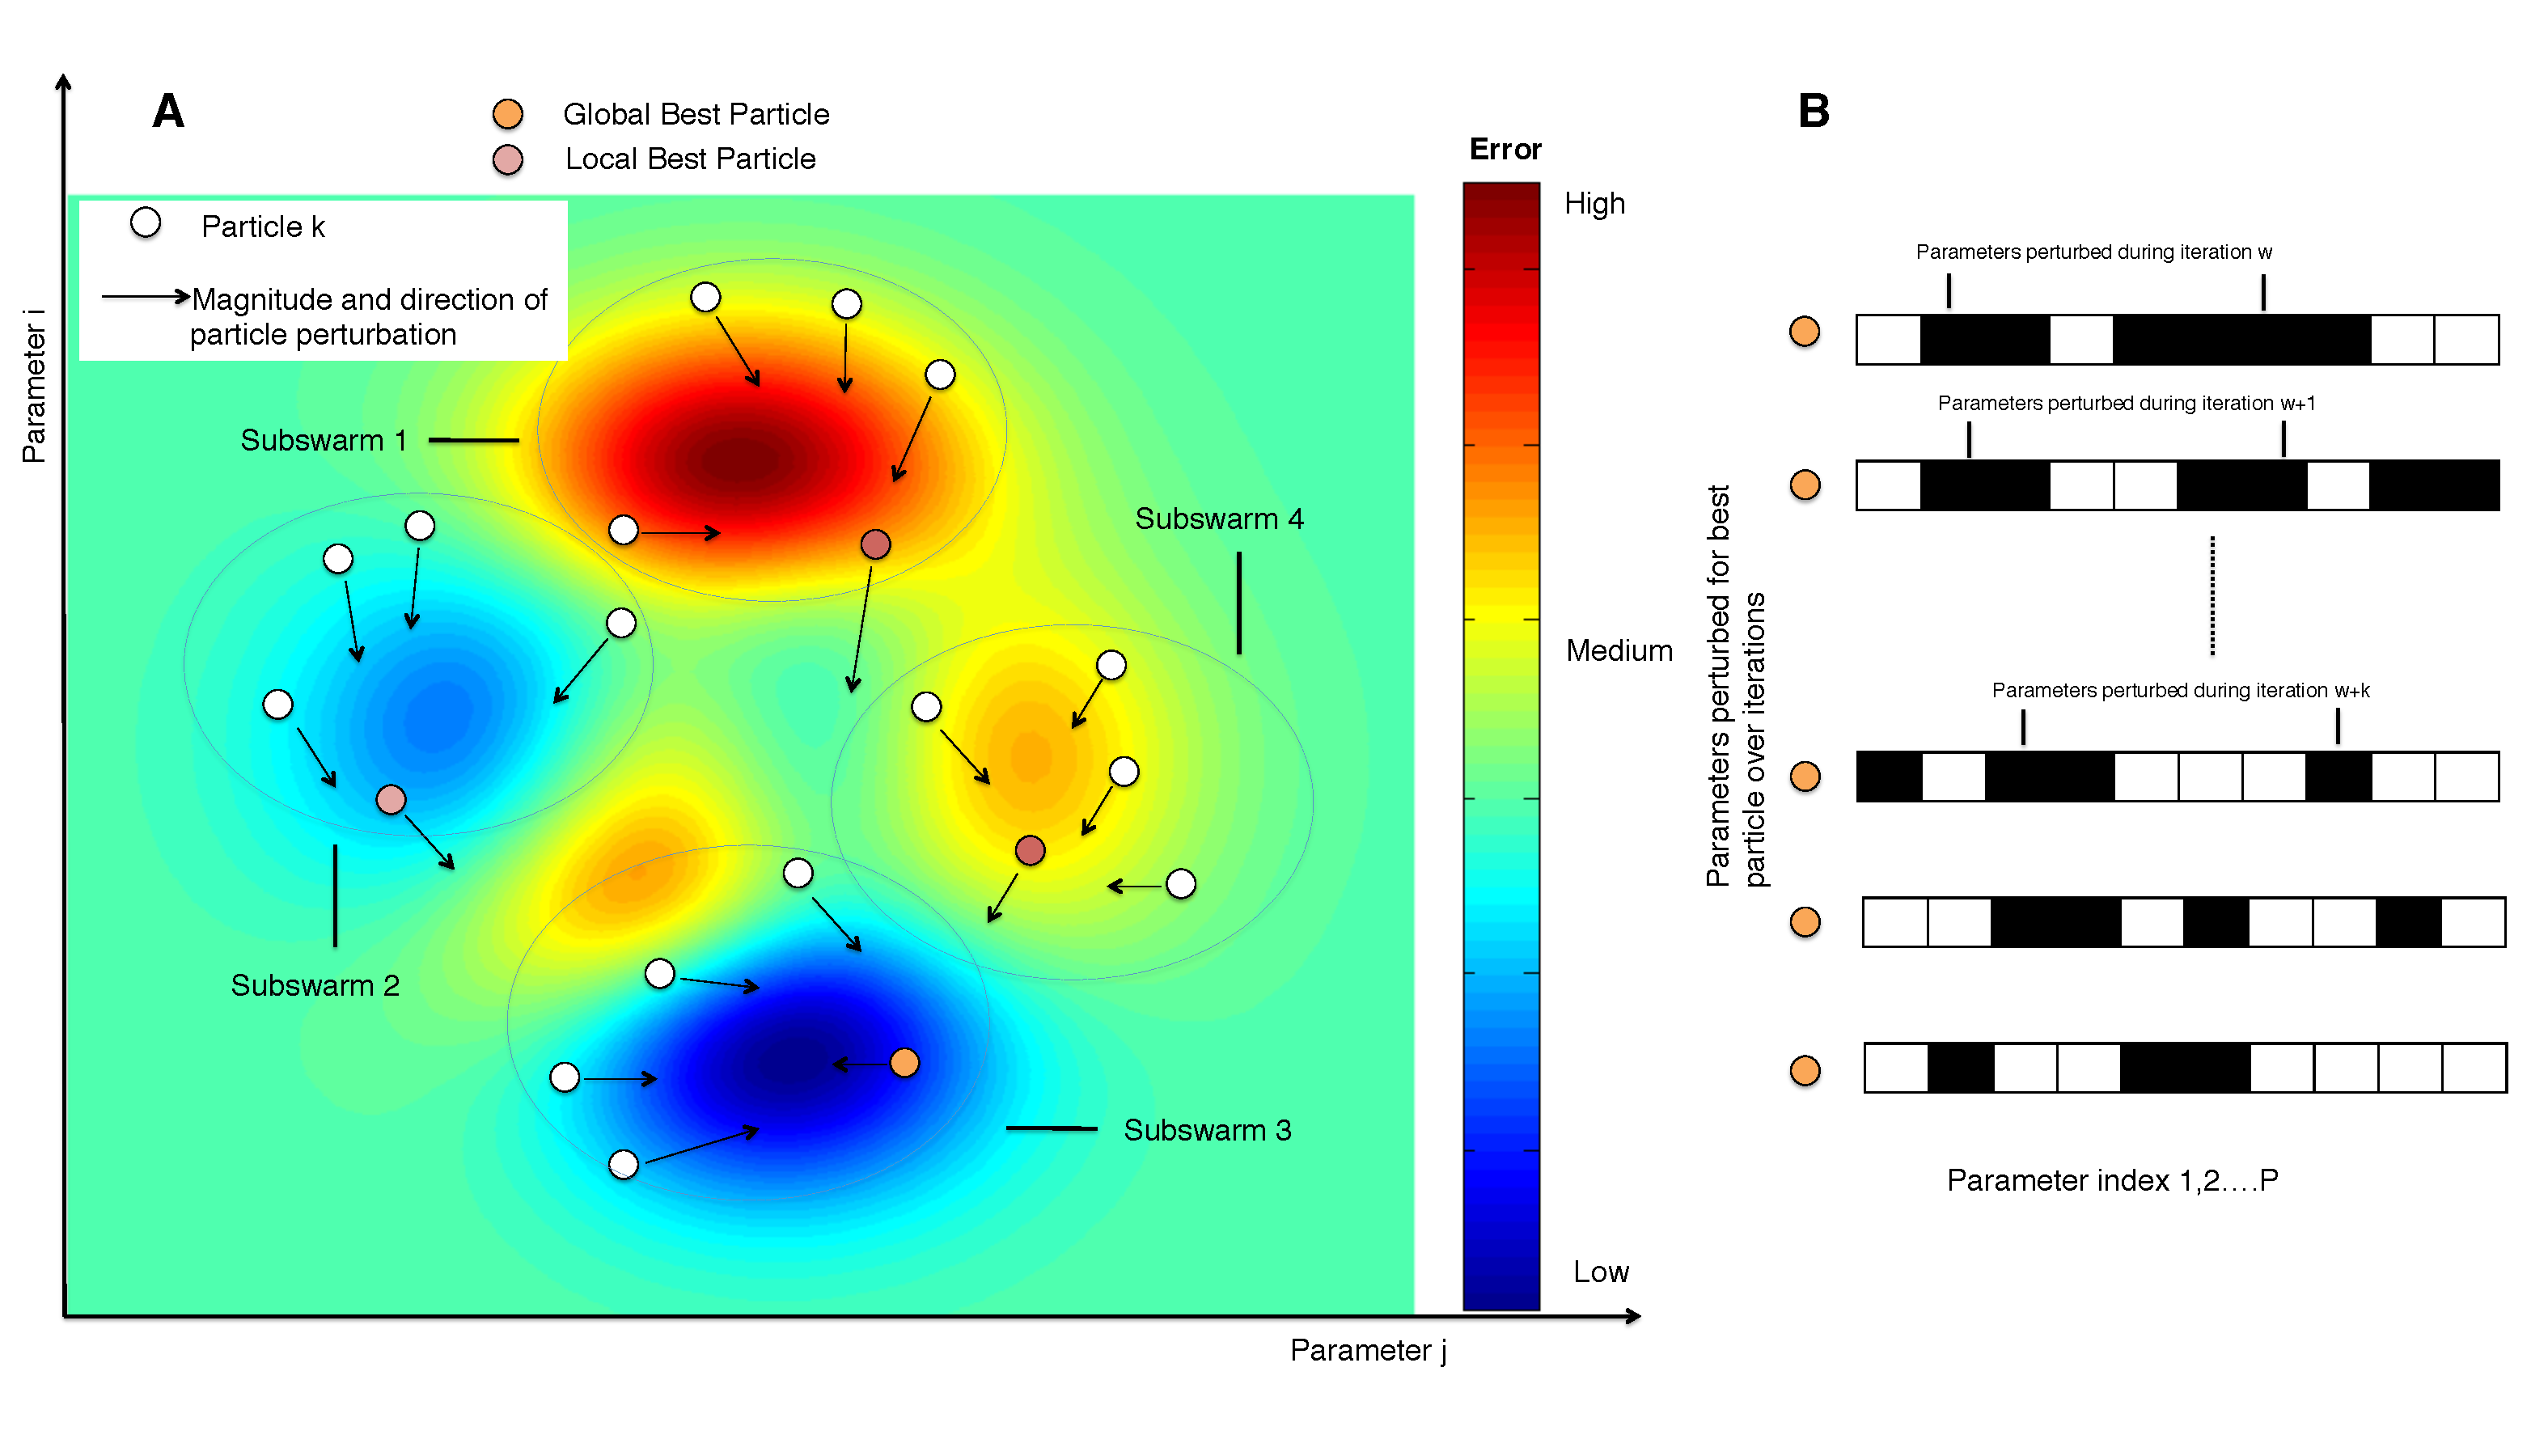
\includegraphics[width=1.0\textwidth]{./figs/Figure_1_Algorithm.pdf}
\caption{Dynamic Optimization with Particle Swarms. \textbf{A}: Each particle represents an N dimensional parameter vector. Particles are given randomly generated initial solutions and grouped into different sub-swarms. Within each swarm the magnitude and direction of the movement a particle is influenced by the position of the best particle and also by its own experience. After every $\mathbf{g}$ number of function evaluations the particles are mixed and randomly assigned to different swarms. When the error due to the global best particle (best particle amongst all the sub-swarms) does not drop over a certain number of function evaluations, the swarm search is stopped and the search switches to a Dynamically Dimensioned Search with global best particle as the initial solution vector or candidate vector.
\textbf{B}: The candidate vector performs a greedy global search for the remaining number of function evaluations. The search neighborhood is dynamically adjusted by varying the number of dimensions that are perturbed (in black) in each evaluation step. The probability that a dimension is perturbed decreases as the number of function evaluations increase. Thus as the evaluations increase the optimality of the solution is preserved.
}\label{fig-algorithm}
\end{figure}

\clearpage

\begin{figure}[ht]
\centering
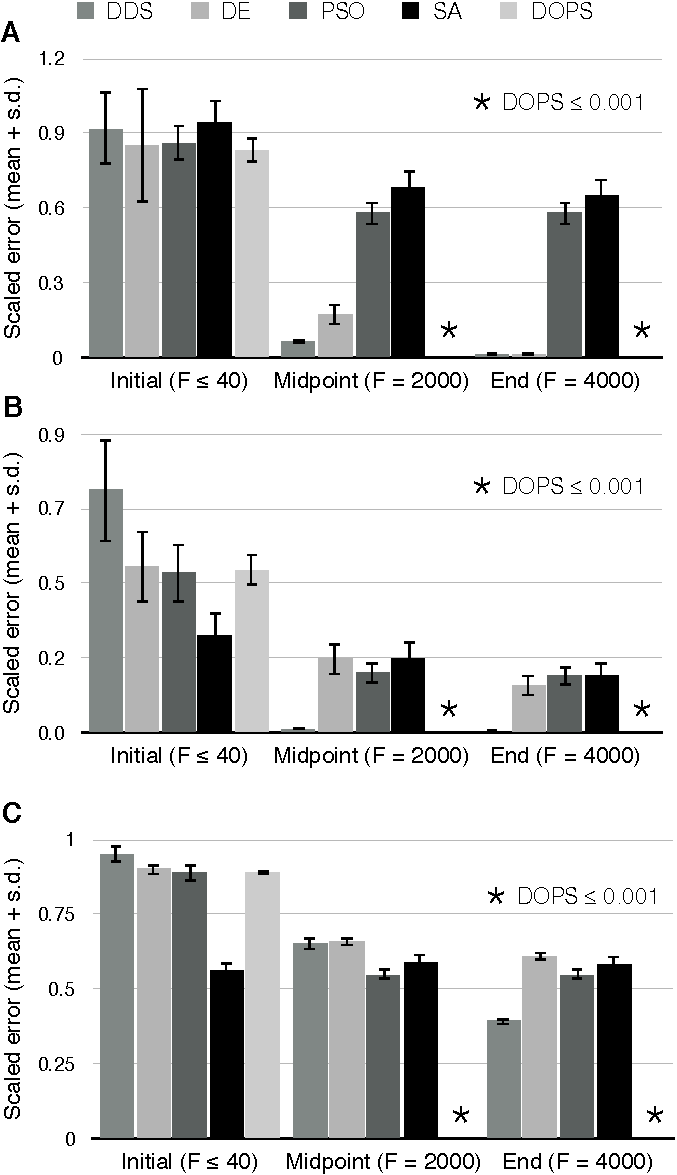
\includegraphics[width=0.7\textwidth]{./figs/Figure_2_TestFunctions-crop.pdf}
\caption{Performance of DOPS and other meta-heuristics for the Ackley and Rastrigin functions.
\textbf{A}: Mean scaled error versus the number of function evaluations for the 10-dimensional Ackley function. DOPS, DDS and DE find optimal or near optimal solutions within the specified number of function evaluations.
\textbf{B}: Mean scaled error versus the number of function evaluations for the 10-dimensional Rastrigin function. DOPS and DDS find optimal or near optimal solutions within the specified number of function evaluations.
\textbf{C}: Mean scaled error versus the number of function evaluations for the 300-dimensional Rastrigin function. DOPS is the only algorithm that finds an optimal or near optimal solution within the specified number of function evaluations. In all cases, the maximum number of function evaluations was 4000. Mean and standard deviation were calculated over 25 trials. }\label{fig-testfunctions}
\end{figure}

\clearpage

\begin{figure}[h]
\centering
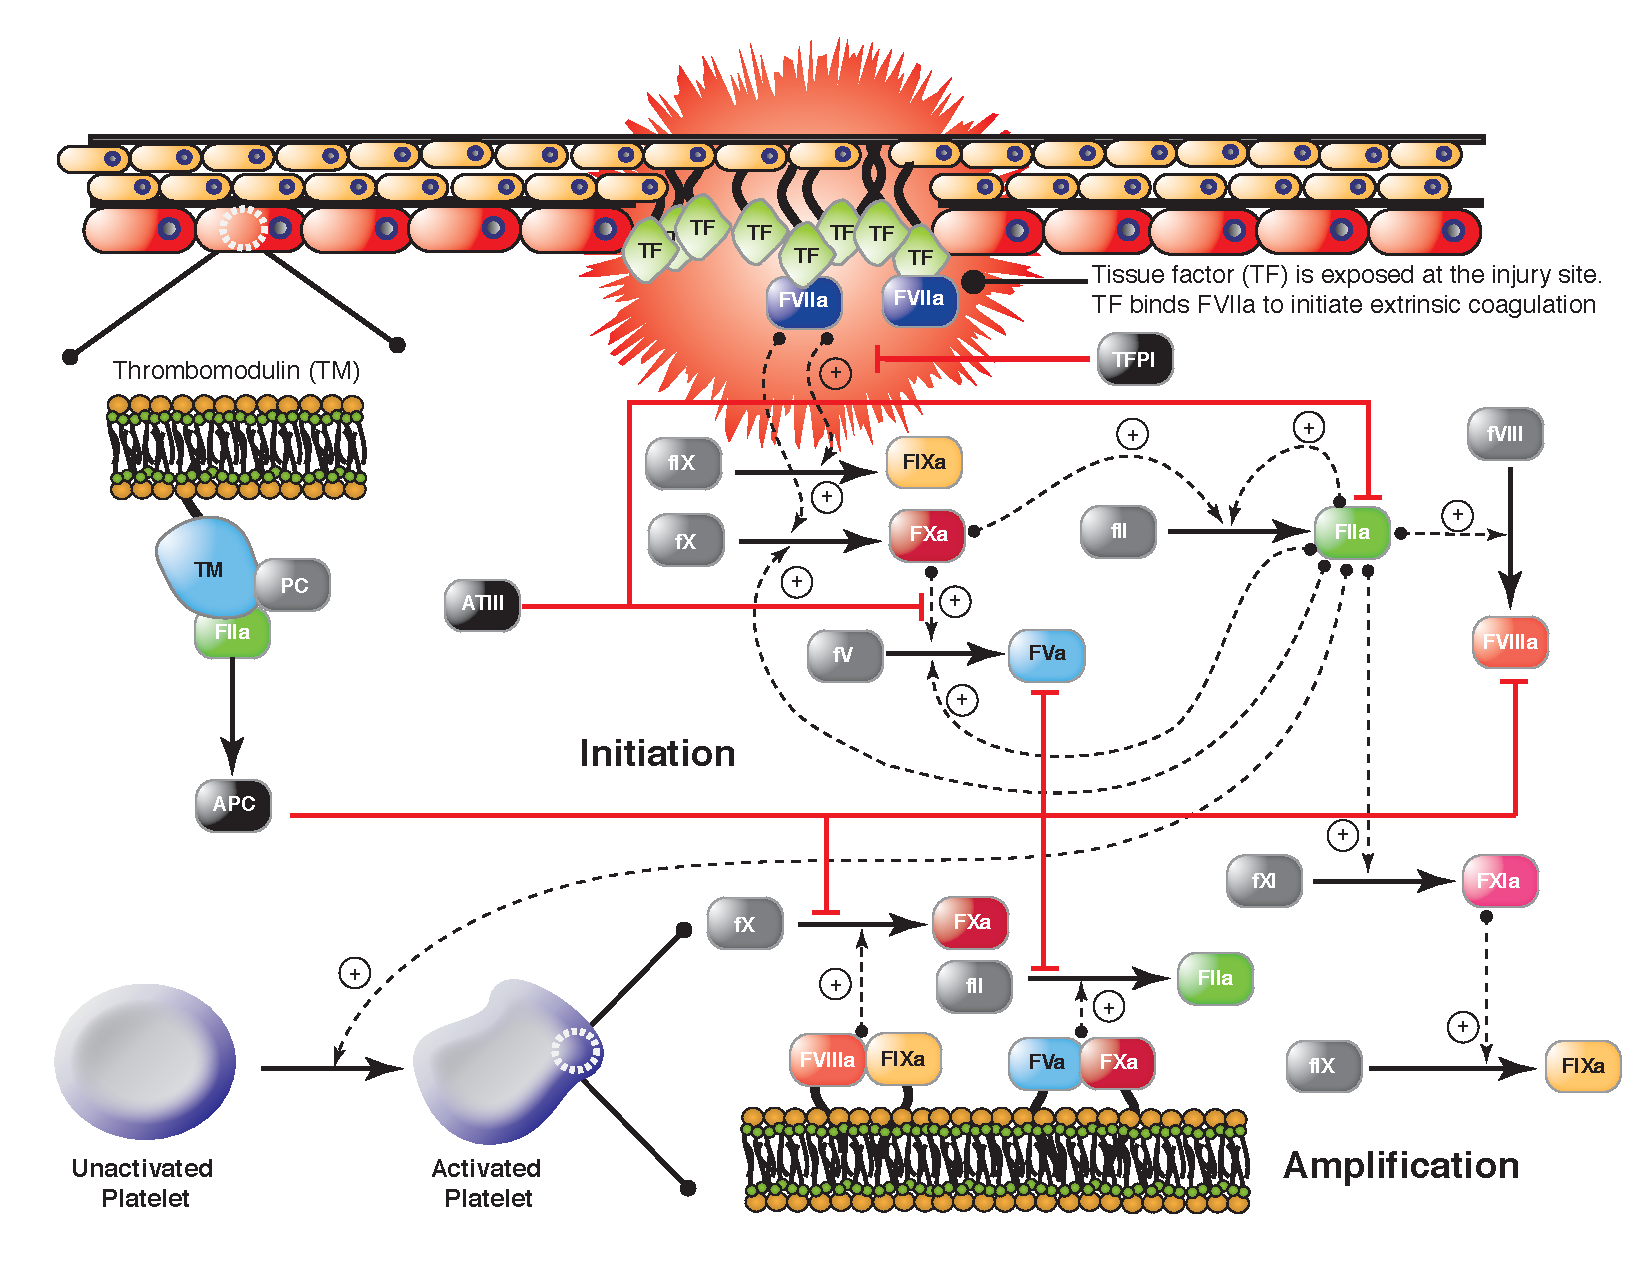
\includegraphics[width=1.00\textwidth]{./figs/Figure_3_Coagulation_v4.pdf}
\caption{Schematic of the extrinsic and intrinsic coagulation cascade\cite{luan2007computationally}. Inactive zymogens upstream (grey) are activated by exposure to tissue factor (TF)  following vessel injury. Tissue factor and activated factor VIIa (FVIIa) form a complex that activates factor X (fX) and IX (fIX). FXa activates downstream factors including factor VIII (fVIII) and fIX. Factor V (fV) is primarily activated by thrombin (FIIa). In addition, we included a secondary fV activation route involving FXa. FXa and FVa form a complex (prothrombinase) on activated platelets that converts prothrombin (fII) to FIIa. FIXa and FVIIIa can also form a complex (tenase) on activated platelets which catalyzes FXa formation.  Thrombin also activates upstream coagulation factors, forming a strong positive feedback ensuring rapid activation. Tissue factor pathway inhibitor (TFPI) downregulates FXa formation and activity by sequestering free FXa and TF-FVIIa in a FXa-dependent manner. Antithrombin III (ATIII)  inhibits all proteases. Thrombin inhibits itself binding the surface protein thrombomodulin (TM). The IIa-TM complex catalyzes the conversion of protein C (PC) to activated protein C (APC), which attenuates the coagulation response by the proteolytic cleavage of fV/FVa and fVIII/FVIIIa. }\label{fig-coagulation-network}
\end{figure}

\clearpage

\begin{figure}[h]
\centering
\includegraphics[width=1.0\textwidth]{./figs/Figure_4_Errors_convergence_v2.pdf}
\caption{Error convergence rates of the five different algorithms on the coagulation model. The objective error is the mean over $N$= 25 trials. DOPS, DDS and SA have the steepest drop in error during first 300 function evaluations. Thereafter the error drop in DDS and SA remains nearly constant whereas DOPS continues to drops further. At the end of 4000 function evaluations DOPS attains the lowest error. The next best estimate using DDS is nearly 3 times greater than the lowest error using DDS.
}\label{fig-convergence}
\end{figure}

\clearpage

\begin{figure}[h]
\centering
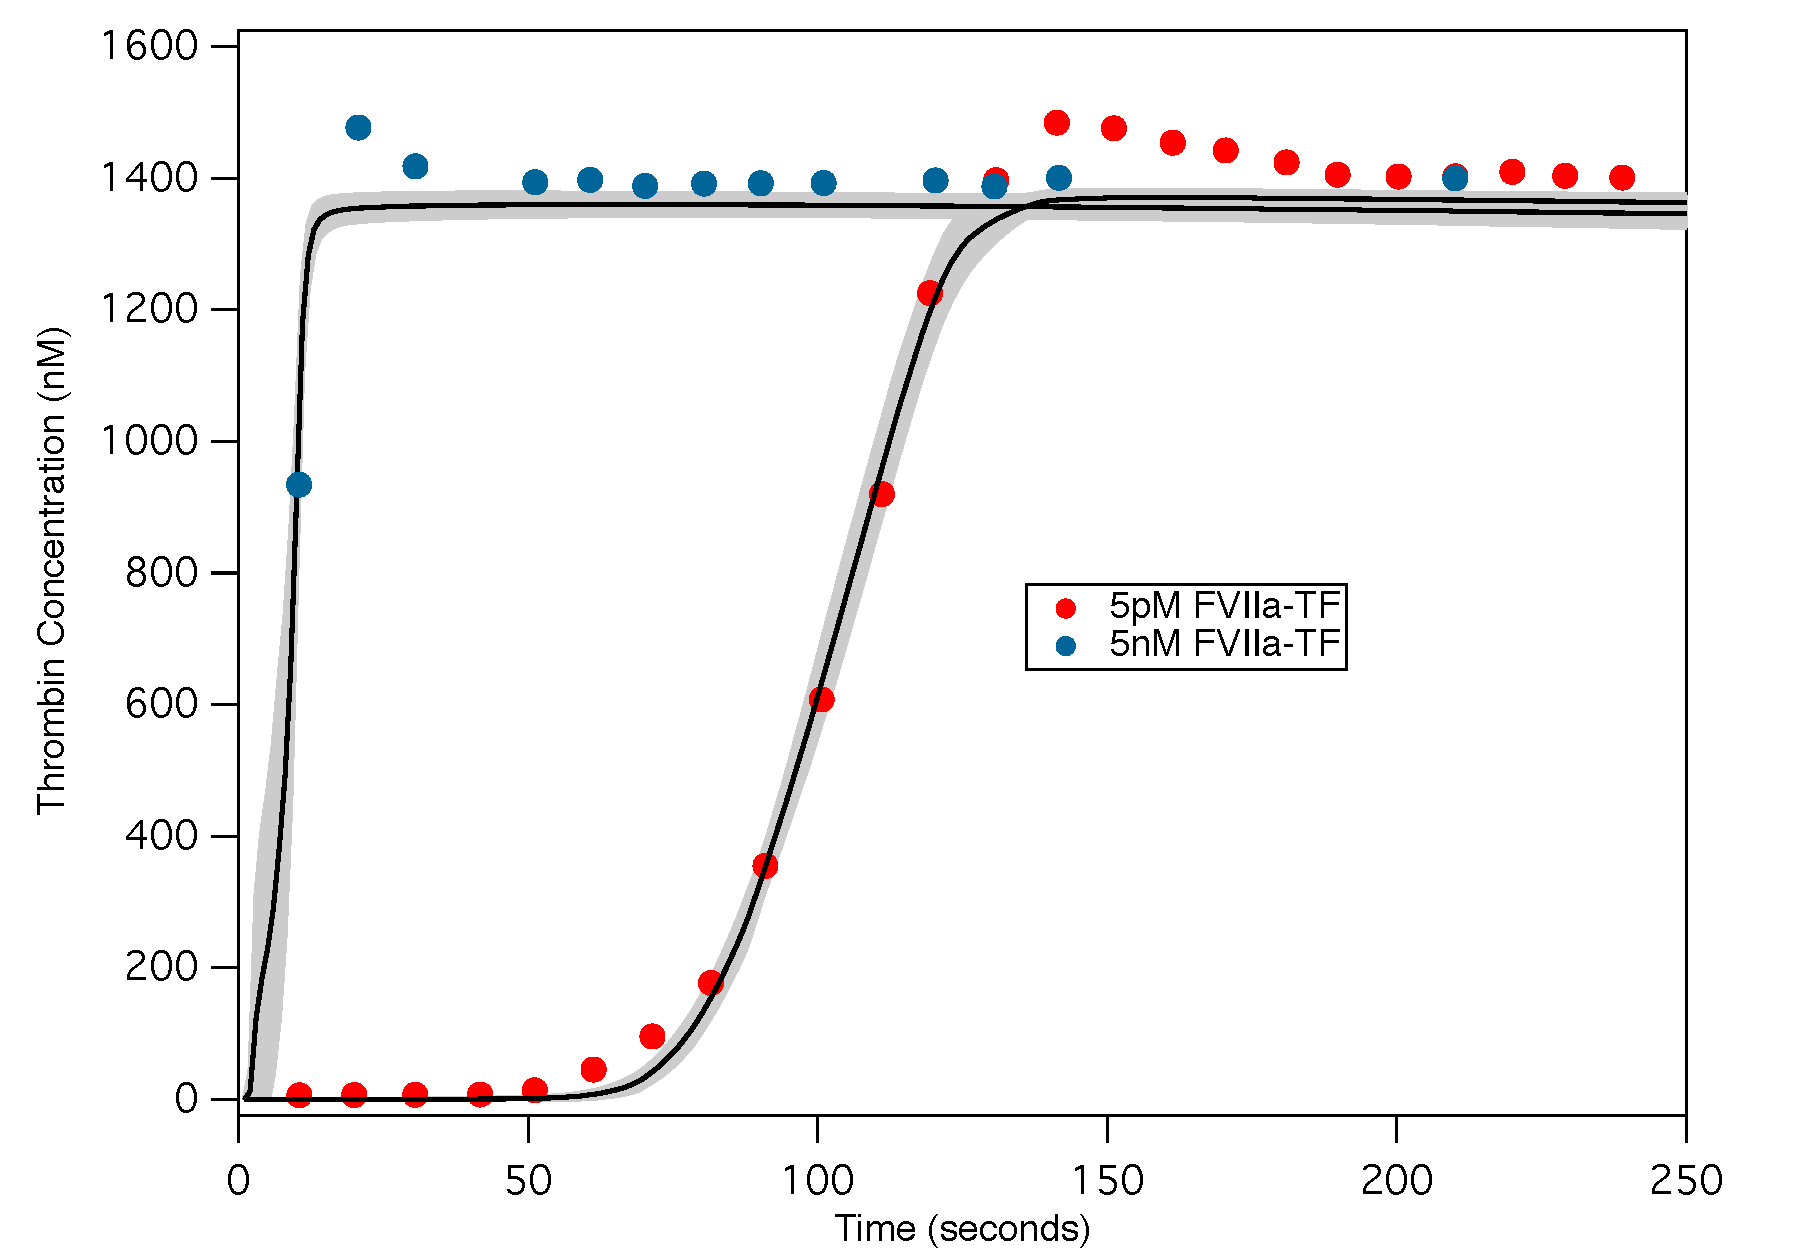
\includegraphics[width=1.0\textwidth]{./figs/Figure_5_Sim_Train_E1_E5.pdf}
\caption{Model fits on experimental data using DOPS. The model parameters were estimated using DOPS. Solid black lines indicate the simulated mean thrombin concentration using parameter vectors from 25 trials. The grey shaded region represents the 99\% confidence estimate of the mean simulated thrombin concentration. The experimental data is reproduced from the synthetic plasma assays of Mann and co-workers. Thrombin generation is initiated by adding Factor TF/VIIa (5nM and 5pM) to synthetic plasma containing 200 $\mu$mol/L of phospholipid vesicles (PCPS) and a mixture of coagulation factors (II,V,VII,VIII,IX,X and XI) at their mean plasma concentrations.
}\label{fig-train}
\end{figure}

\clearpage

\begin{figure}[h]
\centering
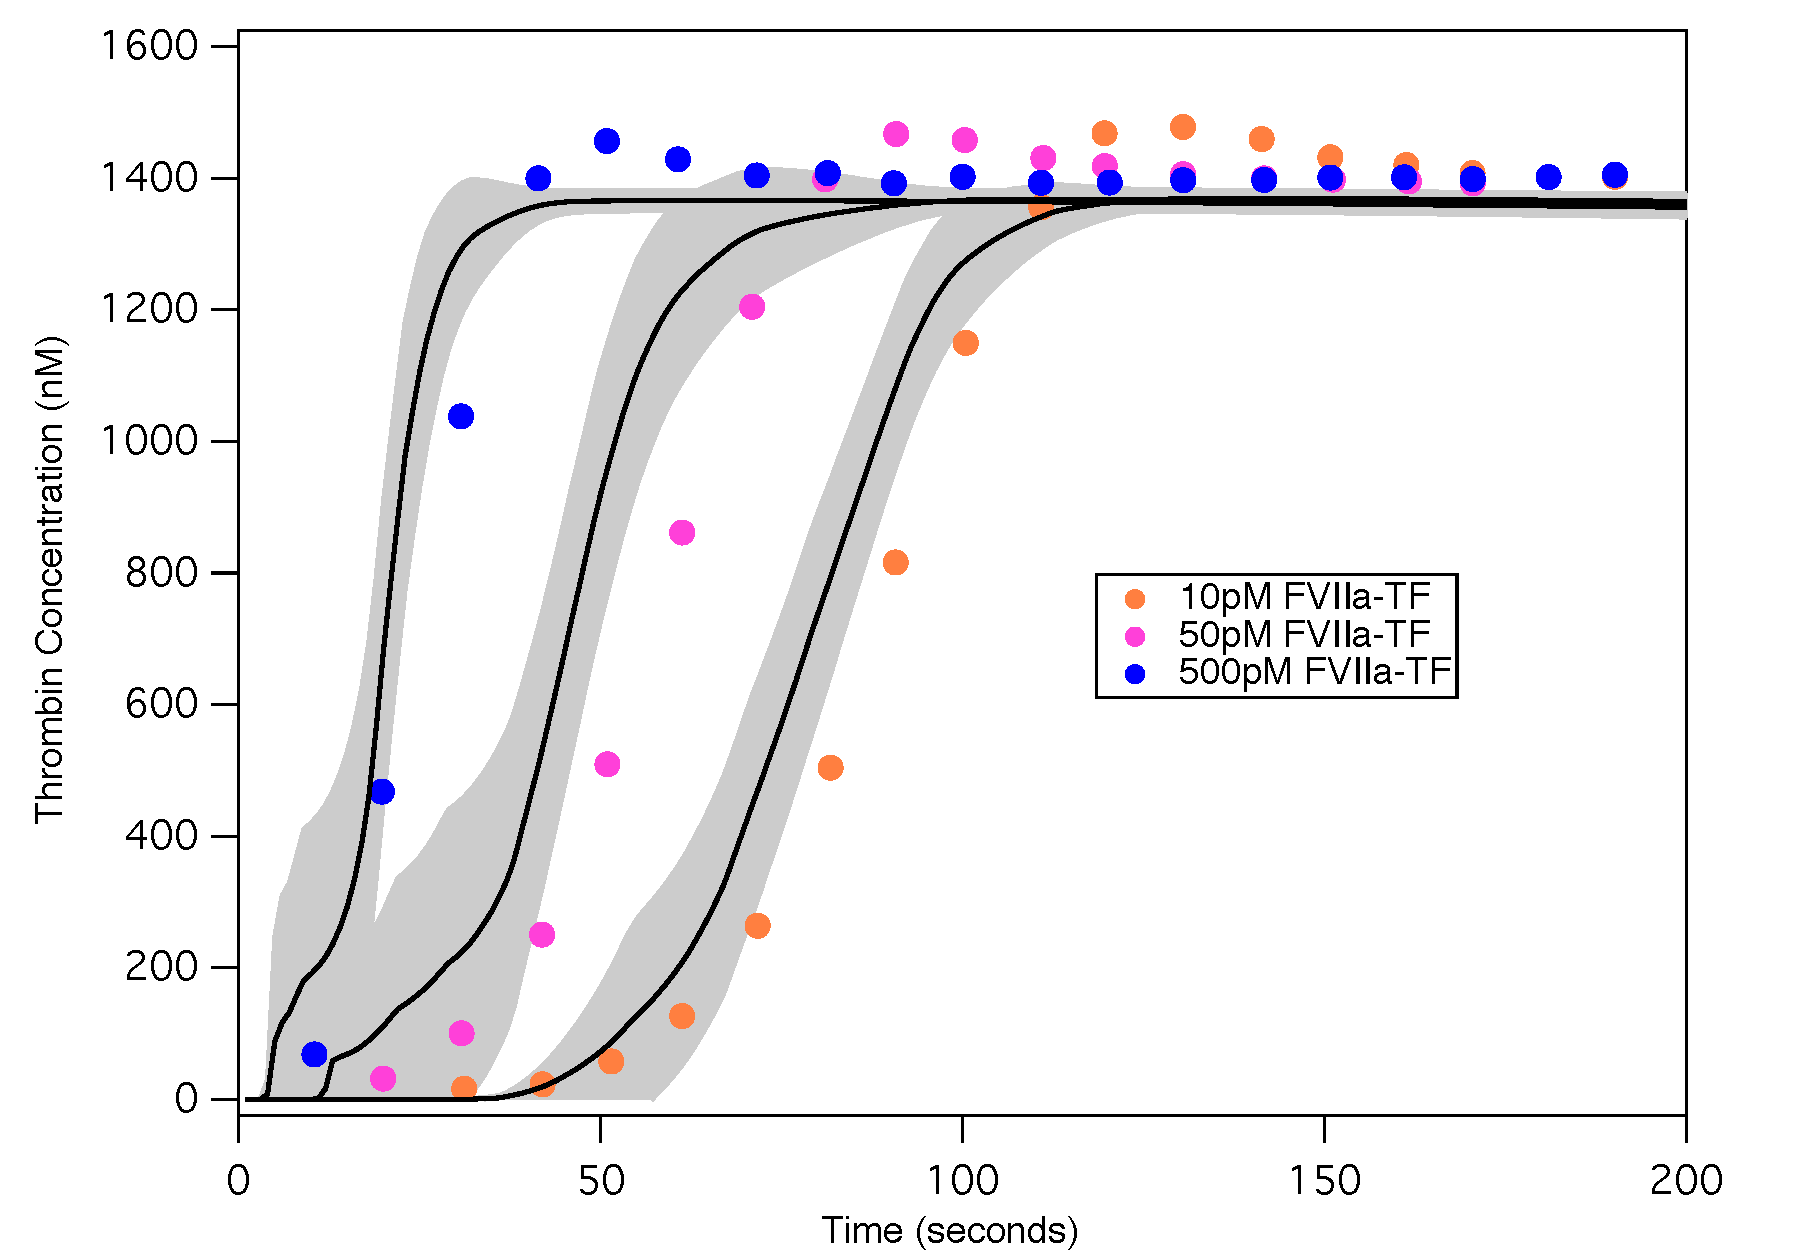
\includegraphics[width=1.0\textwidth]{./figs/Figure_6_Sim_Validate_E2_E4_E6.pdf}
\caption{Model predictions on unseen experimental data using parameters obtained from DOPS. The parameter estimates that were obtained using DOPS were tested against data that was not used in the model training. Solid black lines indicate the simulated mean thrombin concentration using parameter vectors from $N$= 25 trials. The grey shaded region represents the 99\% confidence estimate of the mean simulated thrombin concentration. The experimental data is reproduced from the synthetic plasma assays of Mann and co-workers. Thrombin generation is initiated by adding Factor VIIa-TF (500pM - Blue, 50pM - Pink and 10pM - Orange respectively) to synthetic plasma containing 200 $\mu$mol/L of phospholipid vesicles (PCPS) and a mixture of coagulation factors (II,V,VII,VIII,IX,X and XI) at their mean plasma concentrations.
}\label{fig-validation}
\end{figure}

\clearpage

\begin{figure}[h]
\centering
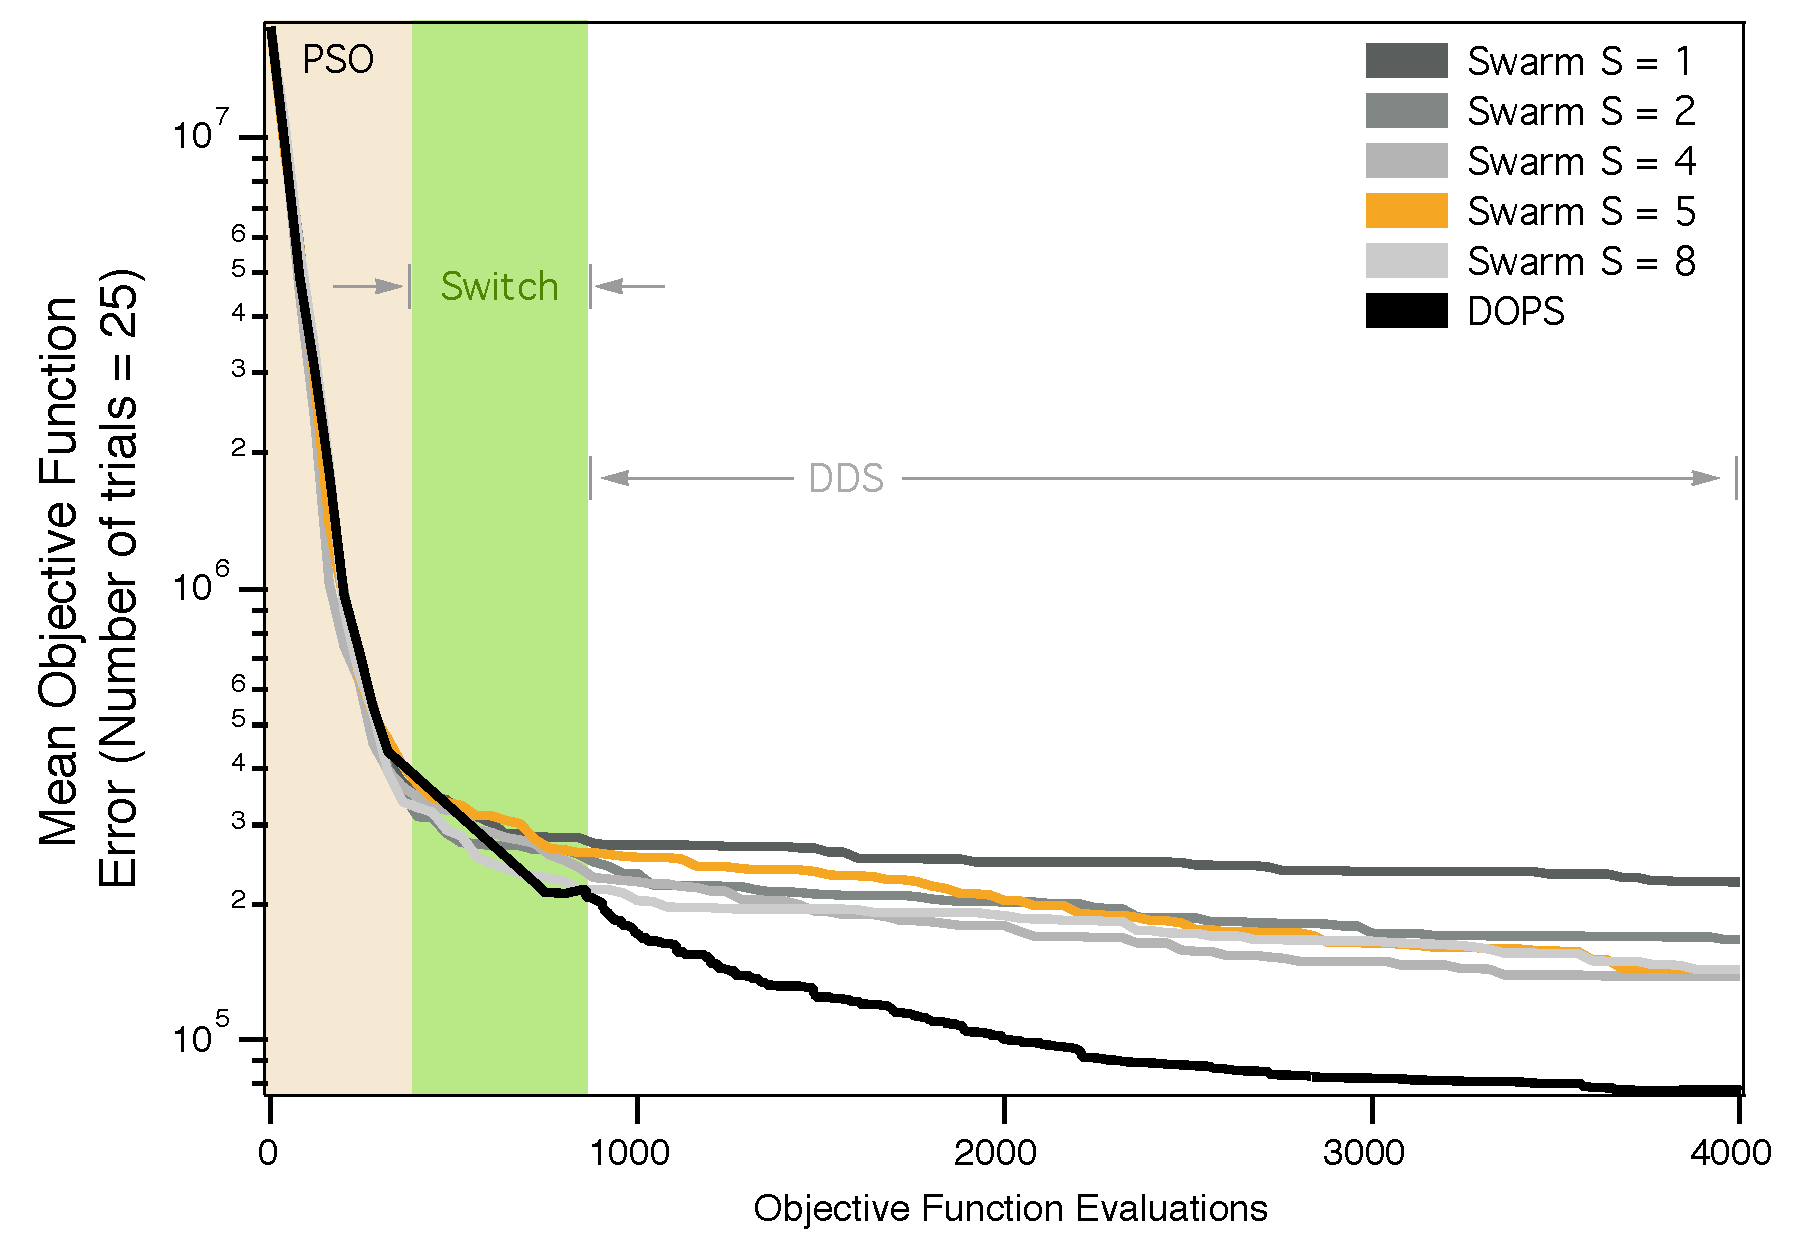
\includegraphics[width=1.0\textwidth]{./figs/Figure_7_ErrorSwarms_v2.pdf}
\caption{DOPS (color:black) begins by using a particle swarm search (color:pale brown) and then dynamically switches (color:green), using an adaptive switching criteria, to the DDS search phase (color:white).
The particle swarm search uses multiple sub-swarms wherein each solution represented by a particle is updated using equation \ref{eqn:update-rule}. The particle update is influenced by the best particle amongst all particles in the sub-swarm and the best solution found by the particle till the current iteration. This update rule however contains no velocity terms. The particle updates continue to happen within the sub-swarms for a certain number of iterations (or function evaluations) after which the sub-swarms are reorganized which is similar to the regrouping strategy described by Zhao et al. \cite{zhao2008dynamic}. DOPS switches out of this PSO phase based on an adaptive switching criteria (color:green) that is a function of error convergence rate. If the error represented by the best particle does not drop for a threshold number of function evaluations, DOPS switches automatically to the DDS search phase. Since the algorithm is stochastic, the switch out can happen at a different function evaluation in each trial. The DDS search then uses the best particle from the PSO search phase as its initial solution or candidate vector. This particle is greedily updated by perturbing a subset of dimensions for the remaining number of function evaluations. The number of dimensions perturbed is a monotonically decreasing function that generally depends on the number of function evaluations within the DDS phase.
We compared the performance of DOPS with multi-swarm searches without DDS to quantify the effect of number of sub-swarms. We used one, two, four, five and eight sub-swarms, with a total of 40 particles divided evenly amongst the swarms. The convergence rates with higher swarm numbers is typically higher but there is no pronounced difference amongst four, five and eight. When the multi-swarm only searches tend to saturate DOPS shows a rapid drop due to a switch to  the DDS phase.
}\label{fig-sub-swarms}
\end{figure}



%\bibitem[Saltelli \em{et~al.}(2010)Saltelli, Annoni, Azzini, Campolongo, Ratto,
  %and Tarantola]{Saltelli:2010}
%Saltelli, A.; Annoni, P.; Azzini, I.; Campolongo, F.; Ratto, M.; Tarantola, S.
%\newblock Variance based sensitivity analysis of model output. Design and
  %estimator for the total sensitivity index.
%\newblock {\em Comput. Phys. Commun.} {\bf 2010}, {\em 181},~259--270.

%\end{thebibliography}

\clearpage

% Supplemental figures -
% Set the S-
\renewcommand\thefigure{S\arabic{figure}}
\renewcommand\thetable{T\arabic{table}}
\renewcommand\thepage{S-\arabic{page}}
\renewcommand\theequation{S\arabic{equation}}

% Reset the counters -
\setcounter{equation}{0}
\setcounter{table}{0}
\setcounter{figure}{0}
\setcounter{page}{1}


\begin{figure}[ht]
\centering
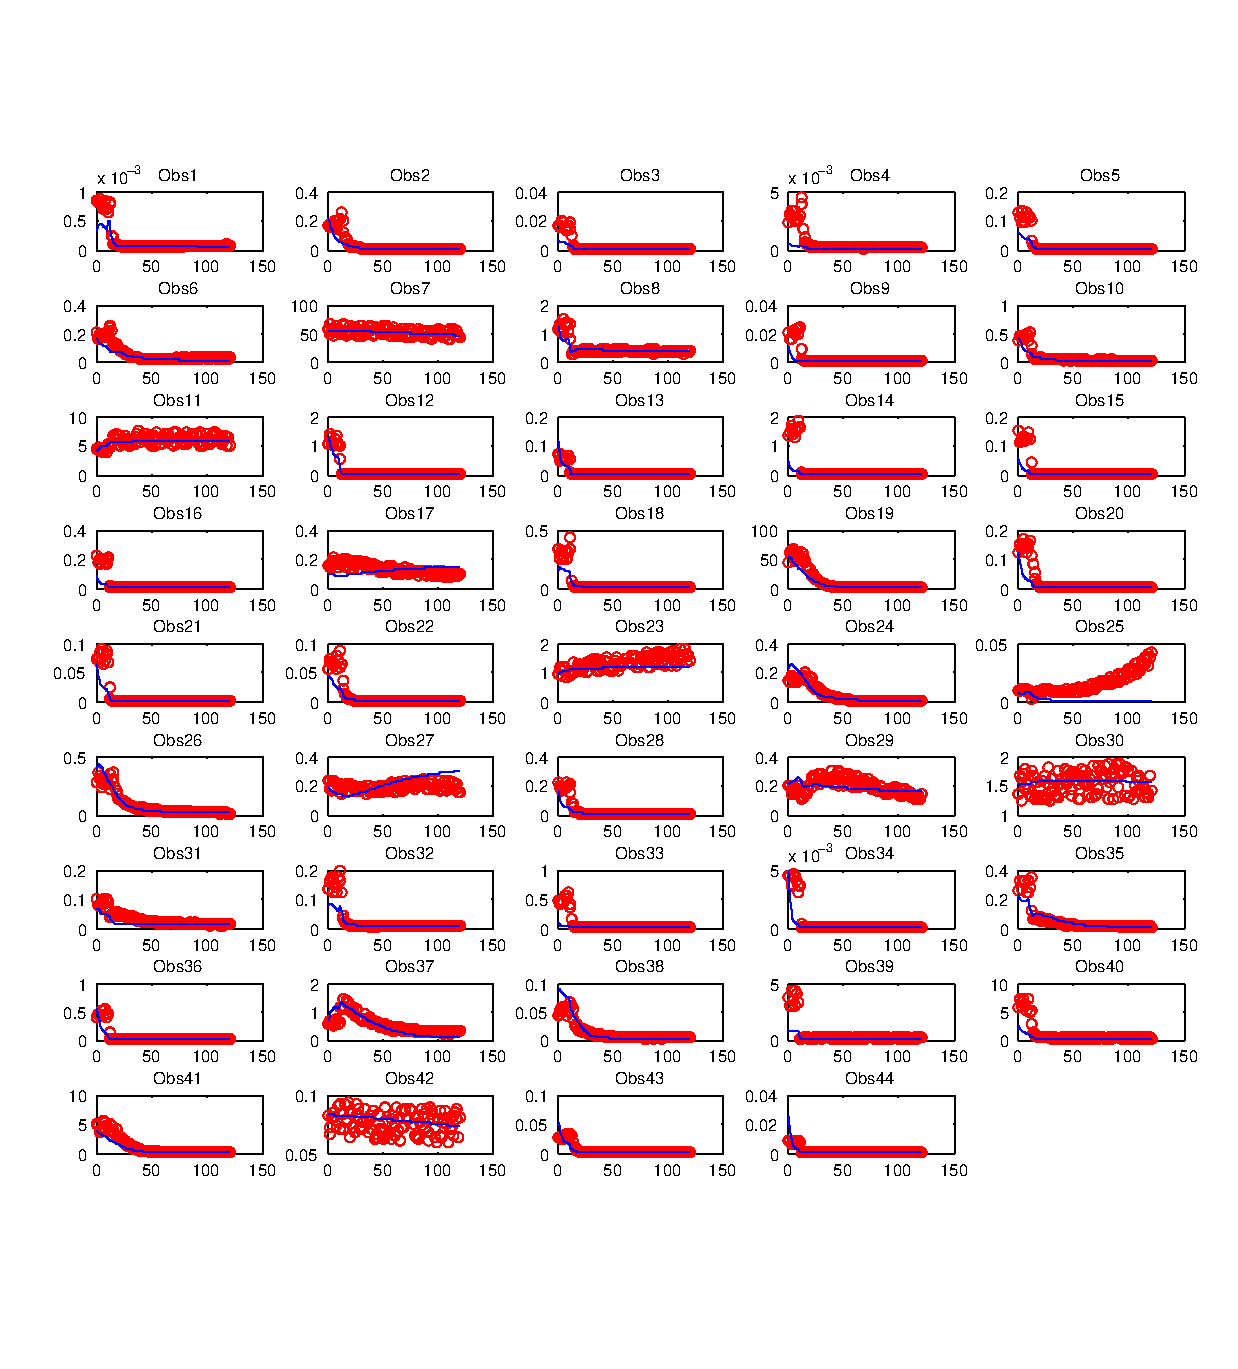
\includegraphics[width=1.00\textwidth]{./figs/Figure_S1_B1_sims.pdf}
\caption{\textbf {(Data fits for Problem B1)} Pseudo-experimental data (red circles) vs. optimal solution obtained using DOPS (solid blue lines) for the 44 observed states. X axis: time [s]; Y axis: metabolite concentrations [mM].
}\label{fig-sims-b1}
\end{figure}

\begin{figure}[ht]
\centering
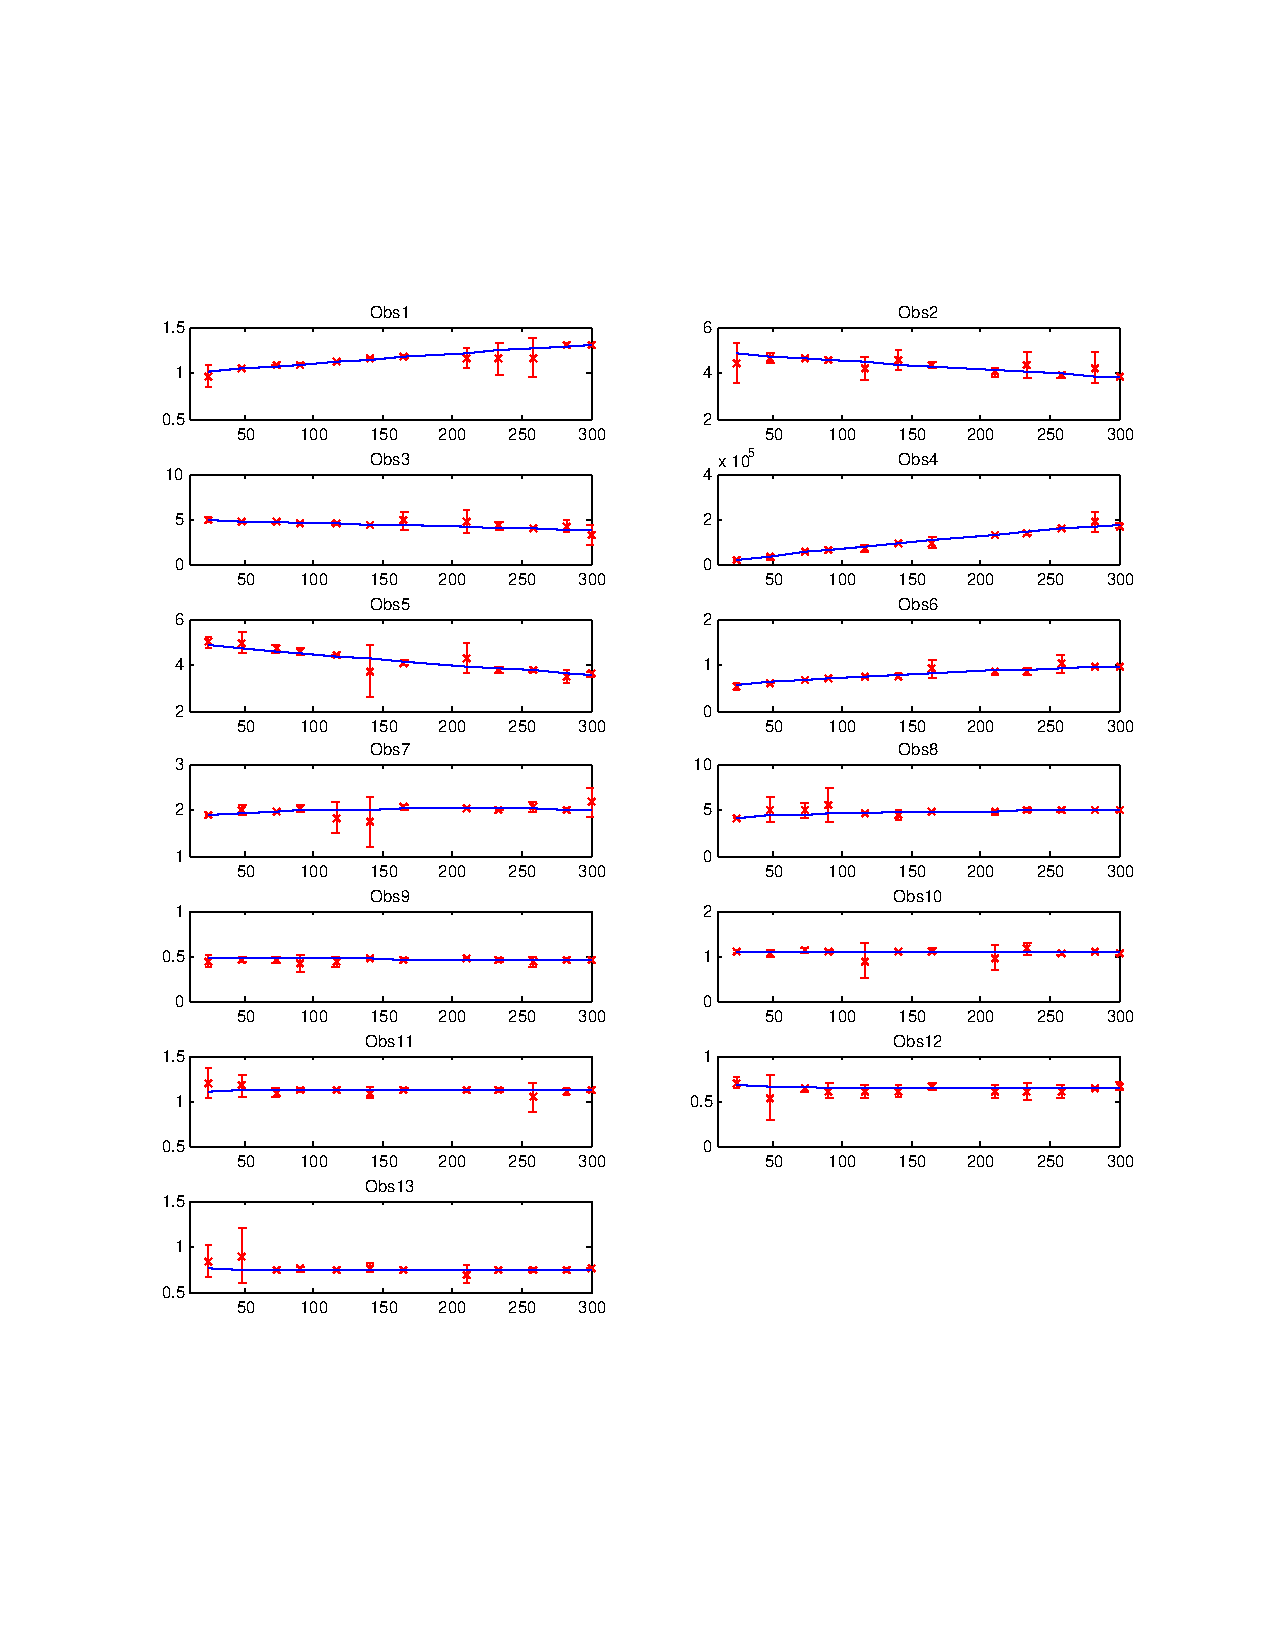
\includegraphics[width=1.00\textwidth]{./figs/Figure_S2_B4_sims.pdf}
\caption{\textbf {(Data fits for Problem B4)} Pseudo-experimental data (red x) vs. optimal solution obtained using DOPS (solid blue lines) for the 13 observed states. X axis: time [s]; Y axis: metabolite concentrations [mM].
}\label{fig-sims-b4}
\end{figure}

\begin{figure}[ht]
\centering
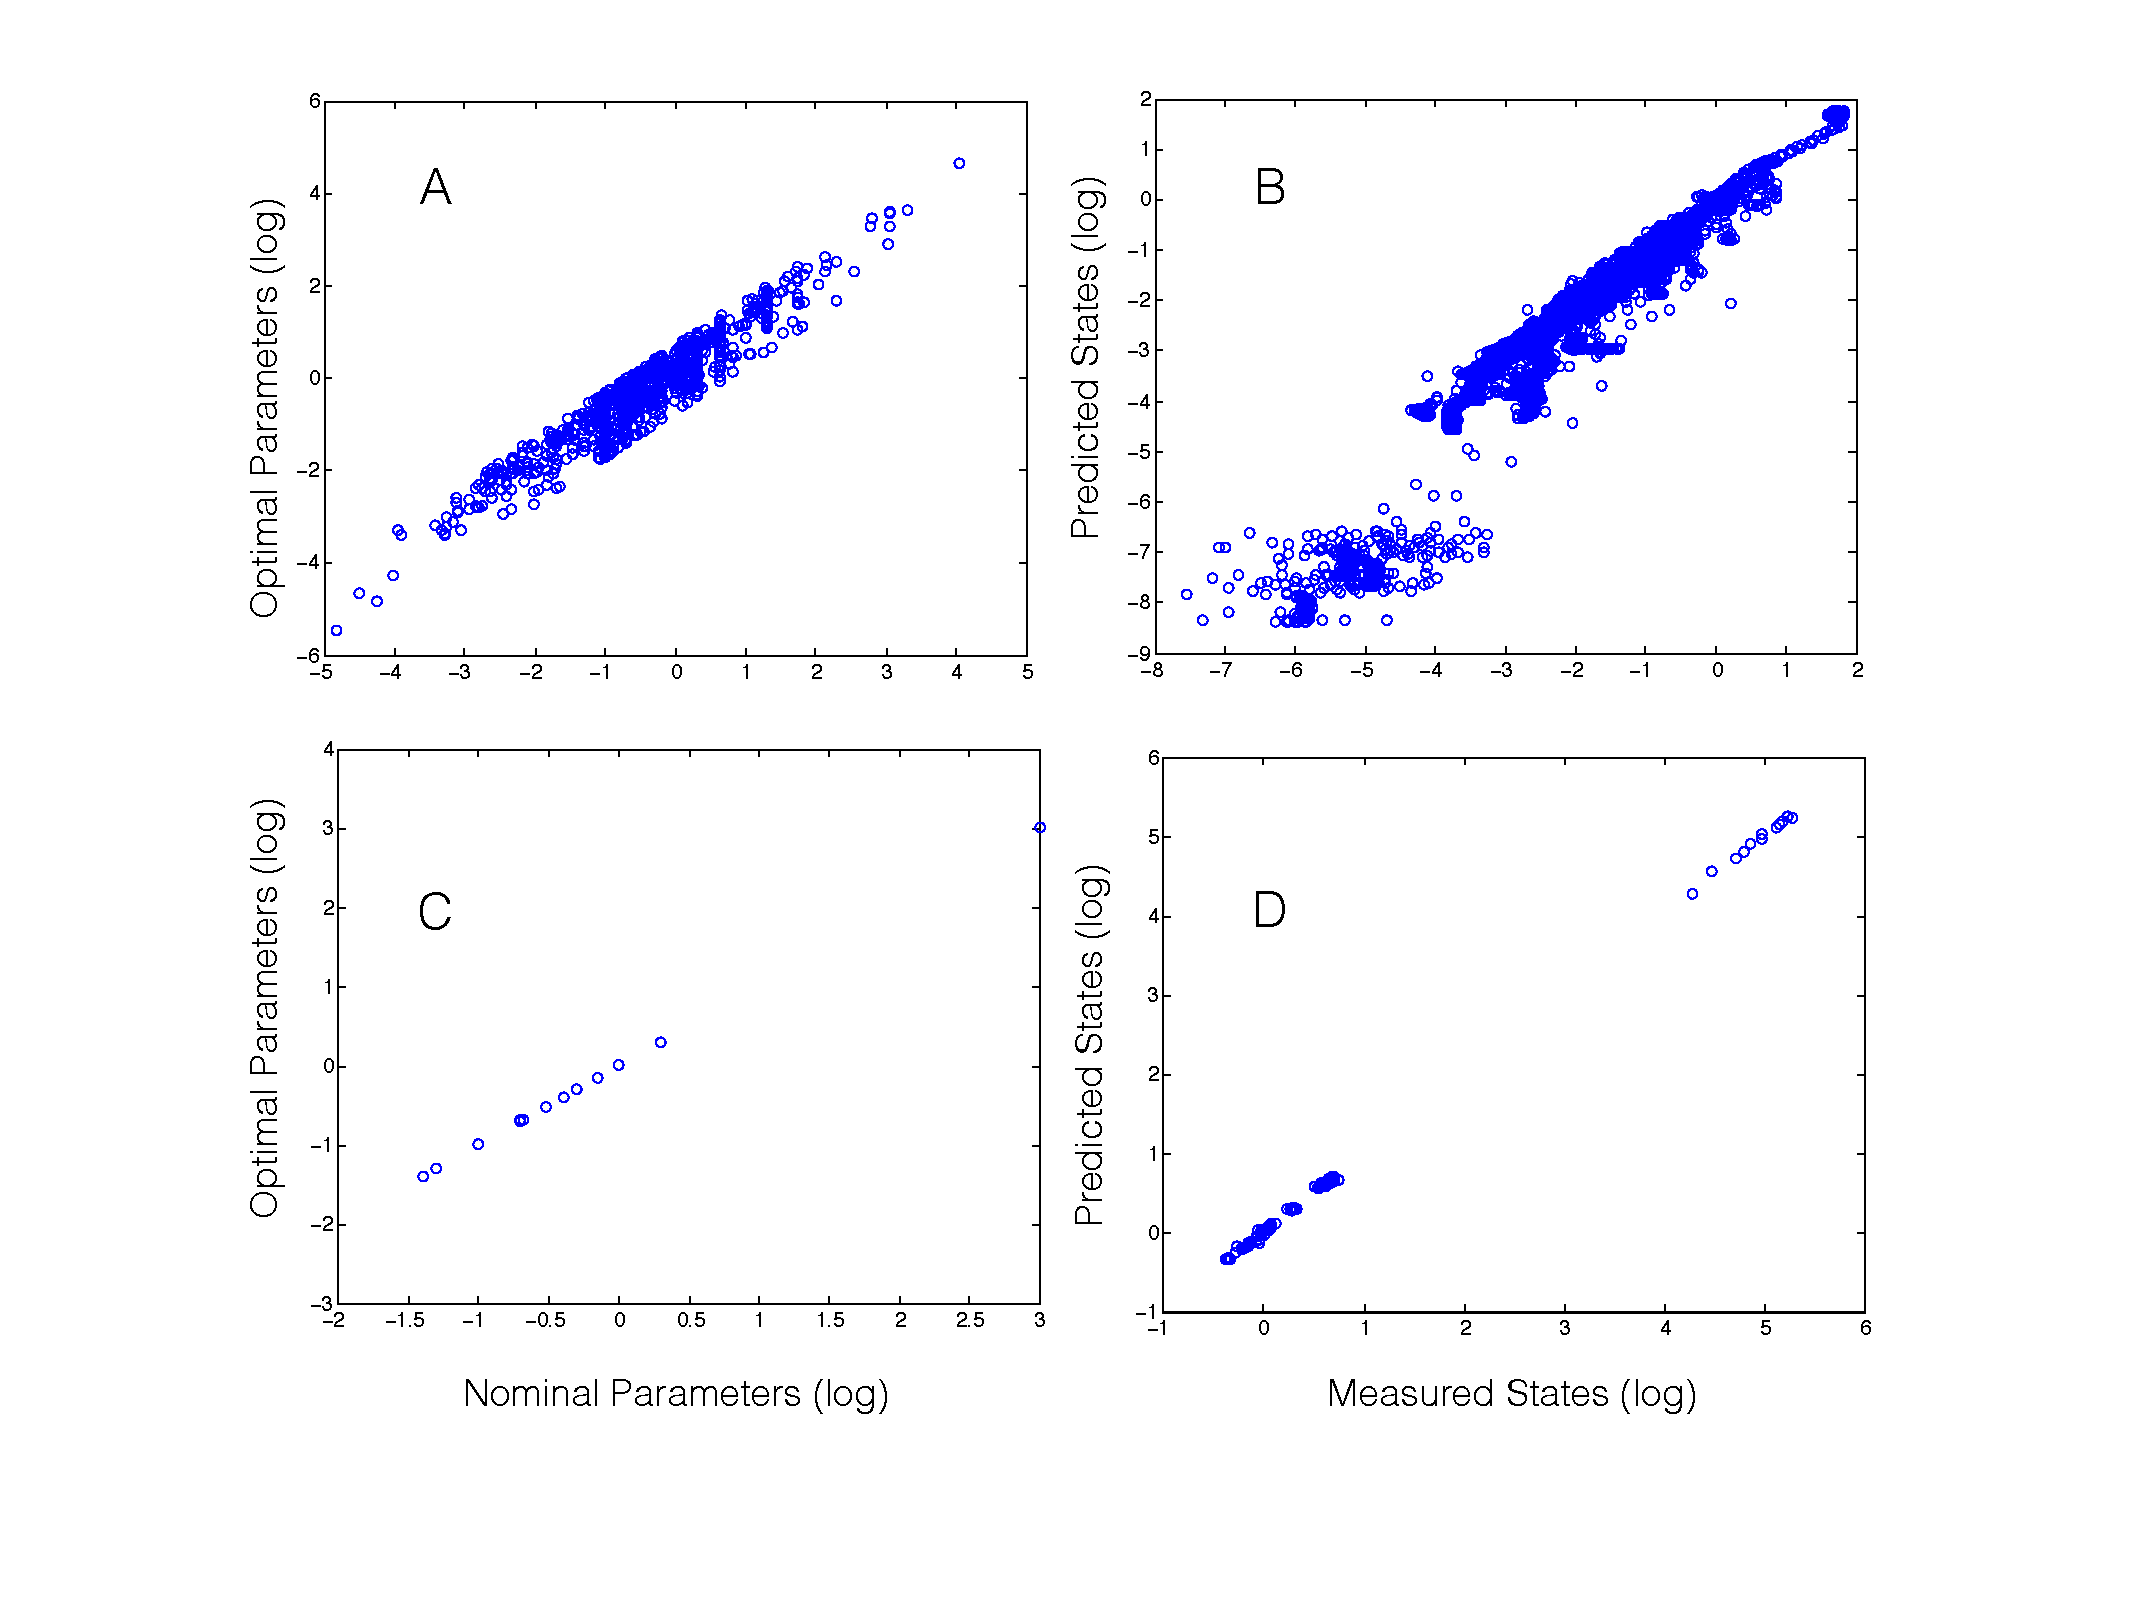
\includegraphics[width=1.00\textwidth]{./figs/Figure_S3_B1_B4_params_measuredstates.pdf}
\caption{ \textbf {(A)} Difference between nominal and optimal parameters for problem B1: Genome wide kinetic model of \textit{S.cerevisiae} with 1759 unknown parameters. \textbf {(B)} Difference between experimental (measured) data and data simulated with optimal parameters for problem B1: Genome wide kinetic model of \textit{S.cerevisiae} with 1759 unknown parameters. \textbf {(C)} Difference between nominal and optimal parameters for problem B4: Metabolic model of Chinese  Hamster Ovary Cells (CHO) cells with 117 parameters. \textbf {(D)} Difference between experimental (measured) data and data simulated with optimal parameters for problem B4: Metabolic model of Chinese  Hamster Ovary Cells (CHO) cells with 117 parameters.
}\label{fig-benchmark}
\end{figure}

\end{document}
